\documentclass[a4paper,8pt,twocolumn]{article}
\usepackage[UTF8]{ctex}
\usepackage{graphicx}
\usepackage{fancyhdr}
\usepackage{amsmath}
\usepackage{subcaption}
\usepackage{float}
\usepackage[
  left=2cm,
  right=2cm,
  top=1.5cm,
  bottom=2.5cm
]{geometry}
\usepackage{siunitx}
\usepackage{booktabs}
\usepackage{enumitem}
\usepackage{array}
\usepackage{tabularx}
\newcolumntype{Y}{>{\centering\arraybackslash}X}
\usepackage{amssymb}
\usepackage{pgfplots}
\usepackage{pgfplotstable}
\pgfplotsset{compat=1.18}

%================ 放电 V-I 曲线统一样式（跨双栏）================
\pgfplotsset{
  viplot/.style={
    width=0.90\textwidth,
    height=0.26\textheight,
    scale only axis,
    grid=major,
    xlabel={电流 $I$ / \si{\micro\ampere}},
    ylabel={电压 $U$ / \si{\volt}},
    title style={font=\small},
    label style={font=\small},
    ticklabel style={font=\scriptsize},
    legend style={font=\scriptsize, at={(0.98,0.98)},
                  anchor=north east, cells={anchor=west}}
  },
  ivplot/.style={
    width=0.90\textwidth,
    height=0.26\textheight,
    scale only axis,
    grid=major,
    xlabel={探针电压 $U_p$ / \si{\volt}},
    ylabel={探针电流 $I_p$ / \si{\micro\ampere}},
    title style={font=\small},
    label style={font=\small},
    ticklabel style={font=\scriptsize},
    legend style={font=\scriptsize, at={(0.02,0.98)},
                  anchor=north west, cells={anchor=west}}
  },
  lnivplot/.style={
    width=0.82\columnwidth,
    height=0.22\textheight,
    scale only axis,
    grid=major,
    xlabel={探针电压 $U_p$ / \si{\volt}},
    ylabel={$\ln(I_p\,/\,\si{\micro\ampere})$},
    title style={font=\small},
    label style={font=\small},
    ticklabel style={font=\scriptsize},
    legend style={font=\scriptsize, at={(0.02,0.98)},
                  anchor=north west, cells={anchor=west}}
  }
}
%=======================================================

\sisetup{
  per-mode=symbol,
  separate-uncertainty=true
}

\title{
  \textbf{\huge 气体放电与等离子体诊断}
}
\author{
  黄雨~24352027\\
  \small 中山大学物理学院~广东~广州
}

\pagestyle{fancy}
\fancyhf{}
\fancyhead[C]{气体放电与等离子体诊断}
\fancyfoot[C]{\thepage}

\begin{document}
\maketitle
\newpage

%%%%%%%%%%%%%%%%%%%%%%%%%%%%%%%%%%%%%%%%%%%%%%%%%%%%%%%%%%%%
\section{实验目的}

\begin{enumerate}
  \item 学习气体放电的原理与物理图像，理解气体放电与金属导电的本质区别；
  \item 掌握放电管的V-I特性曲线及各放电阶段（汤生放电、正常辉光放电、异常辉光放电）的成因；
  \item 观察不同气压下正常辉光放电的外形并作出定性解释；
  \item 了解朗缪尔探针的工作原理，通过I-V特性曲线计算等离子体电子温度$T_e$和等离子体密度$n_e$。
\end{enumerate}

%%%%%%%%%%%%%%%%%%%%%%%%%%%%%%%%%%%%%%%%%%%%%%%%%%%%%%%%%%%%
\section{实验仪器与装置}

\begin{itemize}
  \item 放电管（真空玻璃管，内置阴、阳两极）；
  \item 可调电压电源（最高约950\,V）及多档限流电阻组；
  \item 微安表、伏特表；
  \item 真空泵及气路调压系统（气压范围5—100\,Pa）；
  \item 朗缪尔探针（钨丝，针尖直径$D=0.12$\,mm，针长$L=10$\,mm）；
  \item 探针驱动电源（输出$\pm100$\,V）及数字电压/电流表（精度$\sim1$\,\si{\micro\ampere}）。
\end{itemize}

%%%%%%%%%%%%%%%%%%%%%%%%%%%%%%%%%%%%%%%%%%%%%%%%%%%%%%%%%%%%
\section{实验原理}

\subsection{气体放电V-I特性}

气体本身不存在自由载流子，其导电性依赖外界电离产生的原始载流子和内部碰撞产生的自激载流子。
与金属导电不同，气体的载流子密度随外加电压和气压变化而改变，导致其伏安特性曲线呈现复杂的非欧姆行为。
随外加电压升高，放电依次经历如下阶段：

\begin{enumerate}[label=(\alph*)]
  \item \textbf{汤生放电}：原始电子在电场中加速，通过碰撞电离产生雪崩，
        电流随电压迅速增大，放电尚不稳定；
  \item \textbf{过渡区}：着火后电压骤降，放电从不自持转为自持，经历短暂不稳定过渡；
  \item \textbf{正常辉光放电}：电压保持基本稳定，电流随阴极发射面积扩展而增大，
        放电管出现明暗相间的特征区域（阴极位降区、负辉区、法拉第暗区、正柱区）；
  \item \textbf{异常辉光放电}：阴极面全部覆盖后，电压随电流增大近似线性上升；
  \item \textbf{弧光放电}（本实验设备限制不涉及此阶段）。
\end{enumerate}

\subsection{朗缪尔探针诊断}

将探针插入放电管正柱区（等离子体区），调节探针相对阳极的电位$U_p$，
测量探针电流$I_p$，得到I-V特性曲线。各关键等离子体参数定义及计算方法如下：

\begin{itemize}
  \item \textbf{悬浮电位}$V_f$：$I_p=0$时探针的电位（通常为负值，
        因电子迁移率远大于离子）；
  \item \textbf{等离子体空间电位}$V_p$：电子电流刚开始饱和处的探针电位；
  \item \textbf{电子温度}$T_e$：在$V_f<U_p<V_p$的过渡区，探针收集电流满足
        $I_p\propto\exp(eU_p/kT_e)$，故$\ln I_p$—$U_p$图的斜率为
        \begin{equation}
          k_\text{fit}=\frac{e}{kT_e}
          \quad\Longrightarrow\quad
          T_e\,[\text{eV}]=\frac{1}{k_\text{fit}\,[\si{\per\volt}]};
          \tag{1}
        \end{equation}
  \item \textbf{等离子体密度}$n_e$：由电子饱和电流$I_\text{sat}$计算
        \begin{equation}
          I_\text{sat}=n_e\,e\,A\sqrt{\frac{kT_e}{2\pi m_e}},
          \tag{2}
        \end{equation}
        其中$A=\pi DL$为探针有效面积，$m_e=9.109\times10^{-31}$\,kg为电子质量；
  \item \textbf{德拜长度}：$\lambda_D=\sqrt{\varepsilon_0 kT_e/(n_e e^2)}$，
        要求探针尺寸$D<\lambda_D$以保证测量精度。
\end{itemize}

%%%%%%%%%%%%%%%%%%%%%%%%%%%%%%%%%%%%%%%%%%%%%%%%%%%%%%%%%%%%
\section{实验内容与步骤}

\subsection{气体放电V-I特性曲线测量}

\begin{enumerate}[label=(\arabic*)]
  \item 开启真空泵，将放电腔体抽至5\,Pa以下；
  \item 缓慢旋转气压微调阀，充气至设定值（分别为10、15、20、25\,Pa），稳定后打开电压总电源，调节至约950\,V；
  \item 依次拨动三档限流电阻开关（由最大阻值至最小），每次拨动后记录放电电压$U$和电流$I$；
  \item 在汤生放电、正常辉光放电、异常辉光放电三个典型阶段分别拍摄放电管照片；
  \item 按规程复原仪器（限流电阻、电压源、进气阀、真空泵依次复原）。
\end{enumerate}

\subsection{等离子体诊断}

\begin{enumerate}[label=(\arabic*)]
  \item 调节放电使朗缪尔探针恰好处于正柱区（等离子体区），分别在15、17、19\,Pa下进行测量；
  \item 检查探针电压旋钮归零，打开探针驱动电源；
  \item 缓慢增加探针电压，由$-100$\,V扫至$+100$\,V，逐点记录$U_p$和$I_p$；
  \item 由I-V曲线读取悬浮电位$V_f$和等离子体空间电位$V_p$；
  \item 在过渡区作$\ln I_p$—$U_p$图，线性拟合斜率代入式(1)得$T_e$，
        再由式(2)计算$n_e$；实验结束后按规程复原仪器。
\end{enumerate}

%%%%%%%%%%%%%%%%%%%%%%%%%%%%%%%%%%%%%%%%%%%%%%%%%%%%%%%%%%%%
\section{实验结果与分析}

\subsection{气体放电V-I特性曲线}

图\,\ref{fig:vi_all}\,给出了10、15、20、25\,Pa下放电管的V-I特性曲线。
所有曲线均呈现典型的非欧姆行为：低电流段电压随电流增大而急剧下降（汤生放电到过渡区）；
随后出现一段电压近似不变的平台（正常辉光放电）；本实验中，受限于实验条件，平台区间极不明显，但仍可趋势与理论一致；
高电流段电压随电流增大近似线性上升（异常辉光放电）。
受实验设备电压上限限制，本实验未进入弧光放电阶段。

压力越高，正常辉光放电对应的维持电压越低，最小电压也越低。
这与帕邢定律相符：气压升高时，电子平均自由程缩短，单位路程内碰撞频率增加，
维持自持放电所需的电场强度降低，对应着火电压及正常辉光维持电压均下降。

\begin{figure*}[htbp]
  \centering
  \begin{tikzpicture}
  \begin{axis}[
    viplot,
    title={不同气压下放电管V-I特性曲线},
    legend entries={10\,Pa, 15\,Pa, 20\,Pa, 25\,Pa},
    xmin=0, xmax=3000,
    ymin=270, ymax=720,
  ]
    % ---- 10 Pa ----
    \addplot[mark=none,blue,thick] coordinates {
      (5,403)(5,407)(8,400)(9,402)(9,404)(12,381)(12,386)(15,378)
      (16,381)(19,378)(21,376)(24,372)(26,369)(28,368)(31,362)(33,359)
      (35,357)(40,350)(48,326)(50,323)(53,321)(58,320)(64,321)(70,323)
      (78,325)(83,327)(93,331)(125,343)(142,349)(166,357)(195,367)
      (238,379)(249,382)(260,388)(267,389)(269,392)(291,398)(305,402)
      (311,405)(318,408)(331,412)(339,414)(352,419)(376,425)(392,431)
      (411,437)(437,445)(450,449)(470,455)(488,461)(521,470)(550,478)
      (589,490)(608,496)(640,503)(677,513)(772,536)(921,569)(1042,592)
      (1170,615)(1203,625)(1265,633)(1317,642)(1355,649)(1444,664)(1500,674)
    };
    % ---- 15 Pa ----
    \addplot[mark=none,red,thick] coordinates {
      (3,436)(3,436)(6,404)(7,421)(8,404)(11,395)(11,399)(12,401)
      (14,397)(16,397)(19,390)(22,393)(24,391)(25,392)(26,391)(28,388)
      (29,388)(31,386)(38,378)(40,377)(41,376)(45,373)(52,366)(58,355)
      (68,343)(70,340)(79,334)(117,306)(136,310)(161,314)(192,319)
      (233,327)(246,329)(250,330)(265,332)(269,333)(278,334)(285,336)
      (307,340)(331,344)(342,345)(352,347)(366,349)(375,351)(395,355)
      (422,360)(452,364)(472,369)(517,374)(534,377)(571,384)(600,387)
      (656,394)(684,398)(742,404)(747,406)(790,411)(850,418)(990,436)
      (1233,462)(1400,479)(1632,501)(1707,508)(1800,519)(1840,524)
      (1875,527)(1970,538)(2041,544)
    };
    % ---- 20 Pa ----
    \addplot[mark=none,green!55!black,thick] coordinates {
      (3,438)(3,434)(7,403)(7,415)(7,416)(10,405)(10,410)(12,402)
      (14,402)(16,400)(18,398)(21,395)(22,396)(23,395)(23,395)(26,394)
      (26,394)(28,396)(31,392)(37,381)(38,382)(42,381)(46,378)(53,377)
      (54,372)(63,363)(67,357)(79,348)(112,334)(143,302)(168,302)
      (202,306)(248,312)(262,314)(266,314)(282,317)(285,318)(297,319)
      (300,319)(321,323)(340,325)(345,325)(340,325)(356,327)(360,328)
      (380,331)(410,334)(442,339)(462,341)(502,345)(514,347)(552,351)
      (595,357)(644,361)(677,365)(740,371)(748,372)(786,376)(850,382)
      (1020,397)(1280,420)(1496,438)(1776,455)(1815,460)(1955,469)
      (2044,476)(2124,485)(2240,492)(2355,499)
    };
    % ---- 25 Pa ----
    \addplot[mark=none,orange,thick] coordinates {
      (4,443)(4,445)(8,418)(9,419)(11,410)(12,405)(14,405)(16,406)
      (18,401)(20,402)(23,394)(24,397)(25,395)(25,396)(28,394)(29,390)
      (30,395)(34,389)(40,381)(41,382)(44,380)(50,372)(58,357)(64,354)
      (73,350)(78,348)(88,345)(125,336)(147,334)(185,307)(223,300)
      (275,304)(289,305)(293,305)(313,307)(319,307)(330,308)(336,308)
      (364,311)(379,312)(391,313)(399,314)(423,316)(432,316)(454,318)
      (486,321)(513,324)(539,326)(583,330)(610,332)(645,335)(680,338)
      (739,344)(777,347)(847,352)(859,353)(903,357)(977,362)(1180,376)
      (1509,397)(1756,412)(2077,430)(2177,437)(2330,444)(2390,449)
      (2499,456)(2660,463)(2784,469)
    };
  \end{axis}
  \end{tikzpicture}
  \caption{不同气压下放电管V-I特性曲线。各曲线均依次经历汤生放电（高压低流段）、
           正常辉光放电（电压平台段）和异常辉光放电（线性上升段）三个阶段。}
  \label{fig:vi_all}
\end{figure*}

图\,\ref{fig:vlni_all}\,给出相同数据的V-$\ln I$曲线。以$\ln I$为横轴可以同时展开低电流段（汤生放电）
与高电流段（异常辉光放电），使各阶段的边界更加清晰：汤生放电段电压随$\ln I$近似线性缓降，
正常辉光放电段对应各曲线的电压极小值区域，极小值后电压随$\ln I$线性回升进入异常辉光放电。
随气压升高，极小值对应的放电维持电压逐渐降低，符合帕邢定律。

\begin{figure*}[htbp]
  \centering
  \begin{tikzpicture}
  \begin{axis}[
    width=0.90\textwidth,
    height=0.26\textheight,
    scale only axis,
    grid=major,
    xlabel={$\ln(I\,/\,\si{\micro\ampere})$},
    ylabel={电压 $U$ / \si{\volt}},
    title={不同气压下放电管V-$\ln I$特性曲线},
    title style={font=\small},
    label style={font=\small},
    ticklabel style={font=\scriptsize},
    legend entries={10\,Pa, 15\,Pa, 20\,Pa, 25\,Pa},
    legend style={font=\scriptsize, at={(0.98,0.98)},
                  anchor=north east, cells={anchor=west}},
    xmin=0.8, xmax=8.2,
    ymin=270, ymax=720,
  ]
    % ---- 10 Pa ----
    \addplot[mark=none,blue,thick] coordinates {
      (1.609,403)(1.609,407)(2.079,400)(2.197,402)(2.197,404)
      (2.485,381)(2.485,386)(2.708,378)(2.773,381)(2.944,378)
      (3.045,376)(3.178,372)(3.258,369)(3.332,368)(3.434,362)
      (3.497,359)(3.555,357)(3.689,350)(3.871,326)(3.912,323)
      (3.970,321)(4.060,320)(4.159,321)(4.248,323)(4.357,325)
      (4.419,327)(4.533,331)(4.828,343)(4.956,349)(5.112,357)
      (5.273,367)(5.472,379)(5.517,382)(5.561,388)(5.587,389)
      (5.594,392)(5.673,398)(5.720,402)(5.739,405)(5.761,408)
      (5.802,412)(5.826,414)(5.863,419)(5.930,425)(5.971,431)
      (6.018,437)(6.080,445)(6.109,449)(6.152,455)(6.190,461)
      (6.256,470)(6.310,478)(6.378,490)(6.410,496)(6.461,503)
      (6.518,513)(6.649,536)(6.826,569)(6.949,592)(7.065,615)
      (7.092,625)(7.143,633)(7.183,642)(7.212,649)(7.276,664)(7.313,674)
    };
    % ---- 15 Pa ----
    \addplot[mark=none,red,thick] coordinates {
      (1.099,436)(1.099,436)(1.792,404)(1.946,421)(2.079,404)
      (2.398,395)(2.398,399)(2.485,401)(2.639,397)(2.773,397)
      (2.944,390)(3.091,393)(3.178,391)(3.219,392)(3.258,391)
      (3.332,388)(3.367,388)(3.434,386)(3.638,378)(3.689,377)
      (3.714,376)(3.807,373)(3.951,366)(4.060,355)(4.220,343)
      (4.248,340)(4.370,334)(4.762,306)(4.913,310)(5.081,314)
      (5.257,319)(5.451,327)(5.505,329)(5.521,330)(5.579,332)
      (5.595,333)(5.628,334)(5.652,336)(5.727,340)(5.802,344)
      (5.835,345)(5.863,347)(5.902,349)(5.927,351)(5.979,355)
      (6.044,360)(6.113,364)(6.157,369)(6.248,374)(6.280,377)
      (6.347,384)(6.397,387)(6.486,394)(6.528,398)(6.609,404)
      (6.616,406)(6.672,411)(6.745,418)(6.898,436)(7.117,462)
      (7.244,479)(7.397,501)(7.443,508)(7.496,519)(7.518,524)
      (7.536,527)(7.586,538)(7.621,544)
    };
    % ---- 20 Pa ----
    \addplot[mark=none,green!55!black,thick] coordinates {
      (1.099,438)(1.099,434)(1.946,403)(1.946,415)(1.946,416)
      (2.303,405)(2.303,410)(2.485,402)(2.639,402)(2.773,400)
      (2.890,398)(3.045,395)(3.091,396)(3.135,395)(3.135,395)
      (3.258,394)(3.258,394)(3.332,396)(3.434,392)(3.611,381)
      (3.638,382)(3.738,381)(3.829,378)(3.970,377)(3.989,372)
      (4.143,363)(4.205,357)(4.370,348)(4.718,334)(4.963,302)
      (5.124,302)(5.308,306)(5.513,312)(5.568,314)(5.583,314)
      (5.642,317)(5.652,318)(5.695,319)(5.704,319)(5.771,323)
      (5.829,325)(5.844,325)(5.829,325)(5.875,327)(5.886,328)
      (5.940,331)(6.016,334)(6.091,339)(6.136,341)(6.219,345)
      (6.242,347)(6.313,351)(6.389,357)(6.468,361)(6.518,365)
      (6.607,371)(6.617,372)(6.667,376)(6.745,382)(6.928,397)
      (7.155,420)(7.311,438)(7.482,455)(7.504,460)(7.579,469)
      (7.623,476)(7.661,485)(7.714,492)(7.764,499)
    };
    % ---- 25 Pa ----
    \addplot[mark=none,orange,thick] coordinates {
      (1.386,443)(1.386,445)(2.079,418)(2.197,419)(2.398,410)
      (2.485,405)(2.639,405)(2.773,406)(2.890,401)(2.996,402)
      (3.135,394)(3.178,397)(3.219,395)(3.219,396)(3.332,394)
      (3.367,390)(3.401,395)(3.526,389)(3.689,381)(3.714,382)
      (3.784,380)(3.912,372)(4.060,357)(4.159,354)(4.290,350)
      (4.357,348)(4.477,345)(4.828,336)(4.990,334)(5.220,307)
      (5.407,300)(5.617,304)(5.666,305)(5.680,305)(5.746,307)
      (5.765,307)(5.799,308)(5.817,308)(5.898,311)(5.938,312)
      (5.969,313)(5.990,314)(6.047,316)(6.069,316)(6.118,318)
      (6.186,321)(6.240,324)(6.290,326)(6.368,330)(6.413,332)
      (6.469,335)(6.522,338)(6.606,344)(6.656,347)(6.742,352)
      (6.756,353)(6.806,357)(6.885,362)(7.073,376)(7.319,397)
      (7.471,412)(7.638,430)(7.686,437)(7.753,444)(7.779,449)
      (7.824,456)(7.886,463)(7.931,469)
    };
  \end{axis}
  \end{tikzpicture}
  \caption{不同气压下放电管V-$\ln I$特性曲线。横轴取$\ln I$后低电流段（汤生放电）
           与高电流段（异常辉光放电）均得到充分展开，各放电阶段边界清晰可辨。
           各曲线极小值对应正常辉光放电的维持电压。}
  \label{fig:vlni_all}
\end{figure*}

各气压下不同放电阶段的典型形貌见图\,\ref{fig:disch10}—图\,\ref{fig:disch25}。
汤生放电阶段放电管内仅有微弱、弥散的辉光；进入正常辉光放电后，可见明显的明暗相间分区
（负辉区、法拉第暗区、正柱区等）；进入异常辉光放电后，辉光覆盖全部阴极面，亮度增强。

\begin{figure*}[htbp]
  \centering
  \begin{subfigure}{0.32\textwidth}
    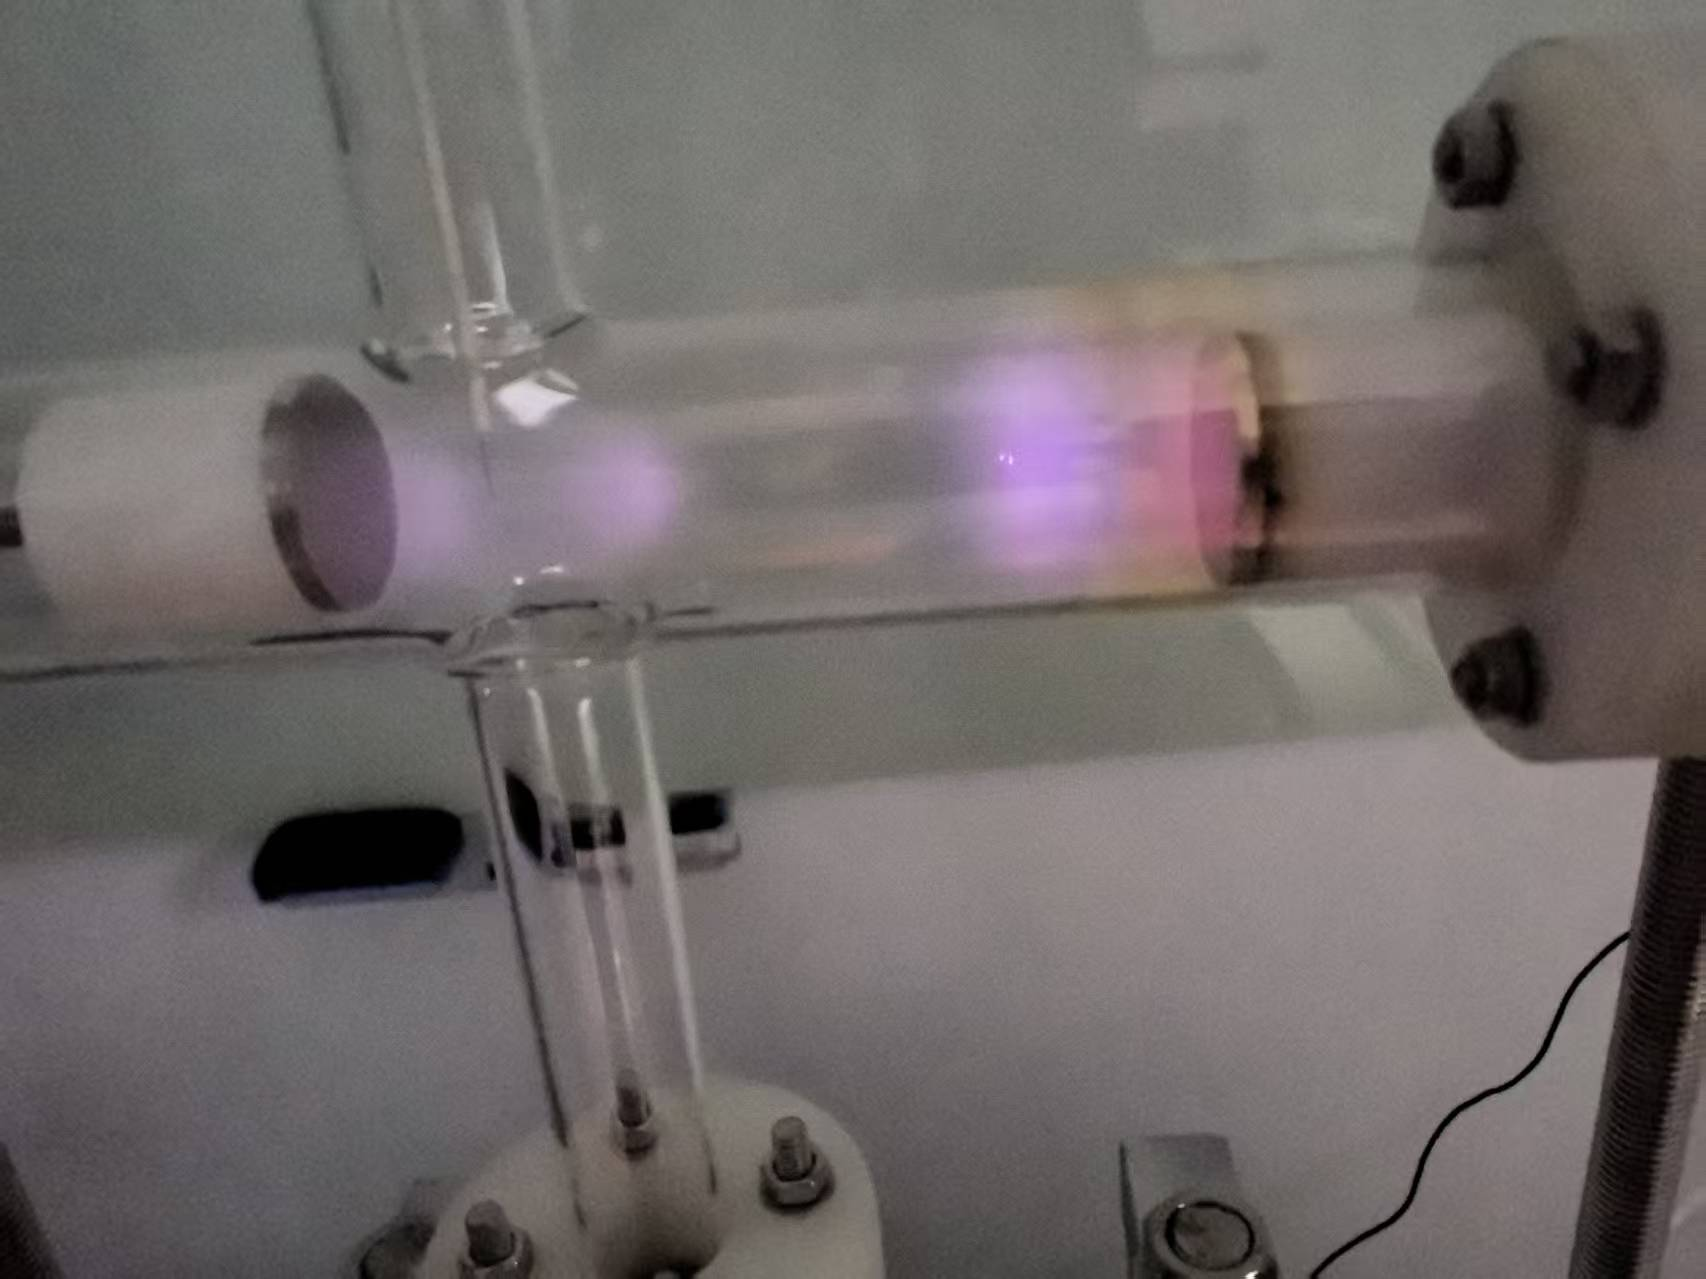
\includegraphics[width=\linewidth,keepaspectratio]{10Pa_汤生放电.jpg}
    \caption{汤生放电}
  \end{subfigure}\hfill
  \begin{subfigure}{0.32\textwidth}
    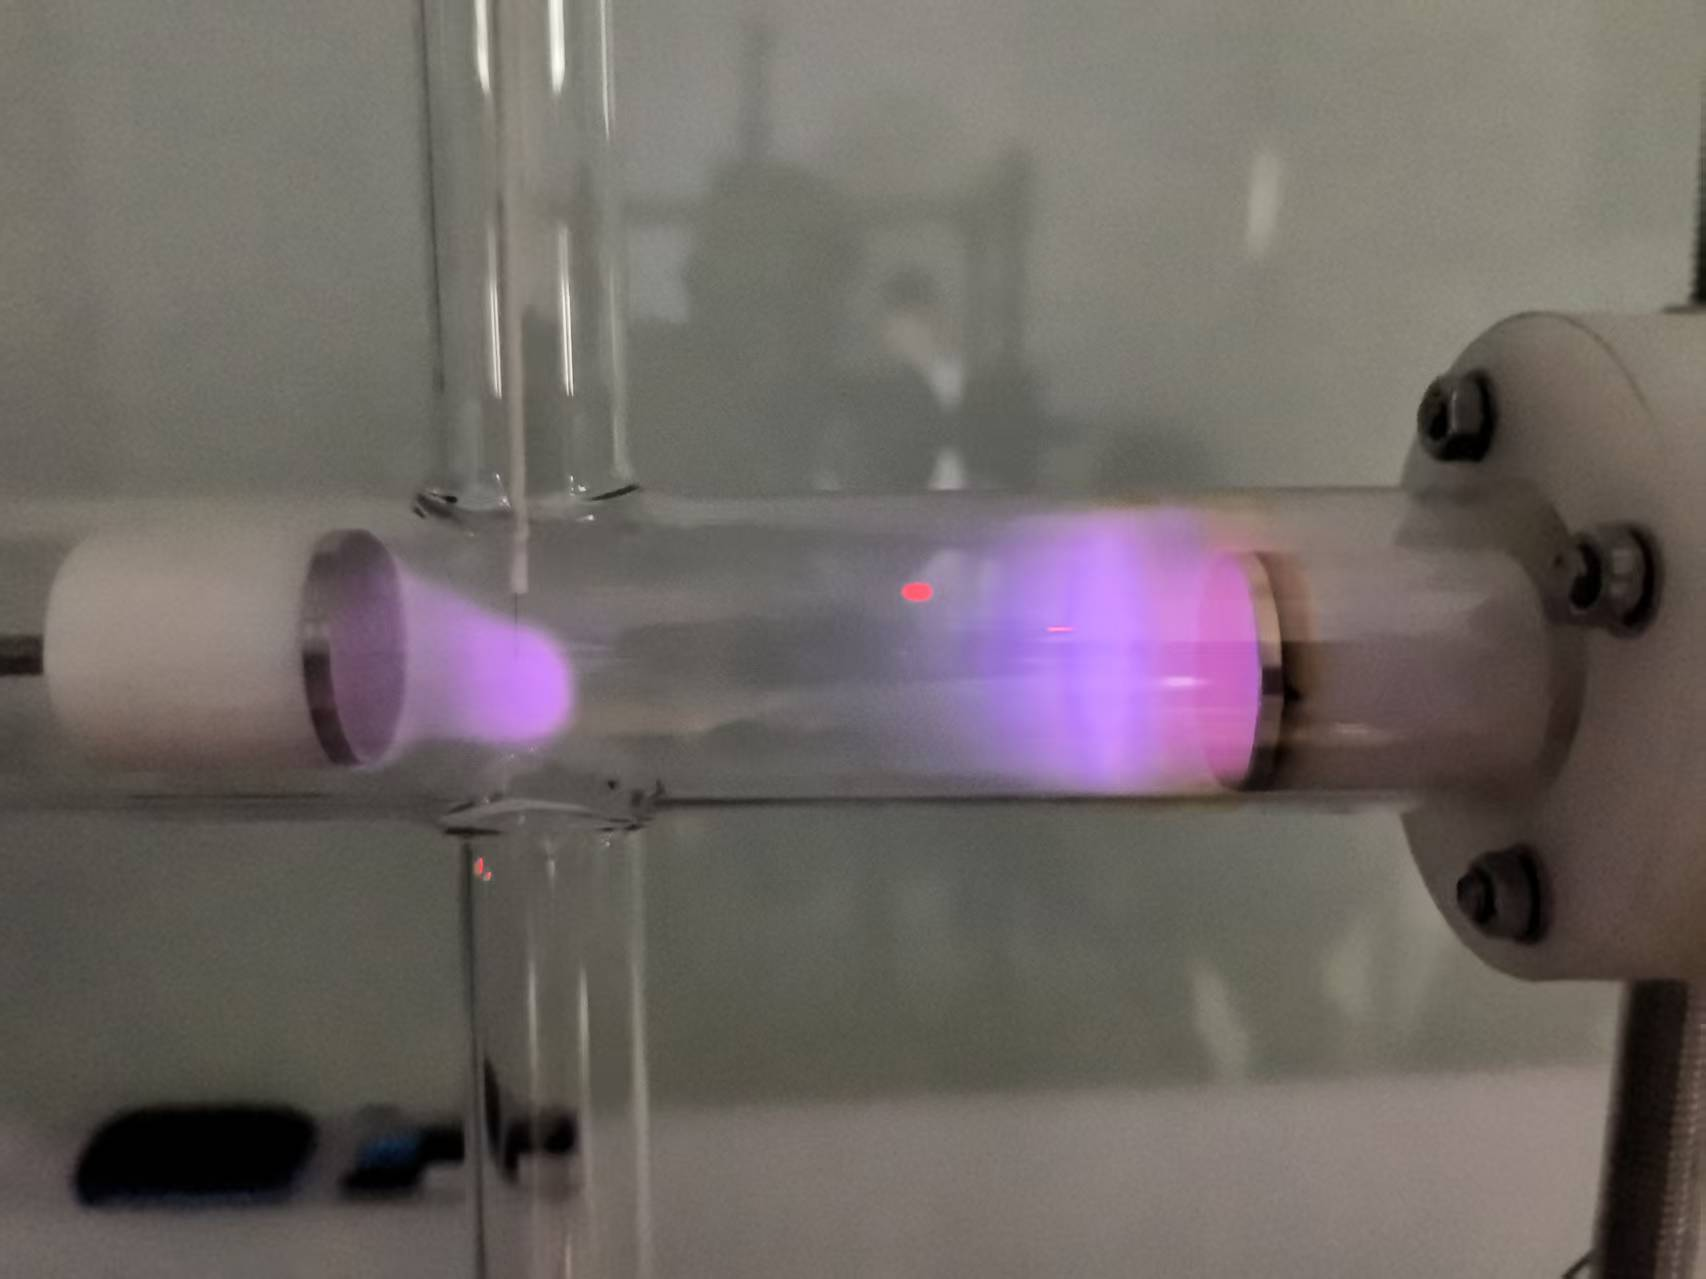
\includegraphics[width=\linewidth,keepaspectratio]{10Pa_正常辉光放电.jpg}
    \caption{正常辉光放电}
  \end{subfigure}\hfill
  \begin{subfigure}{0.32\textwidth}
    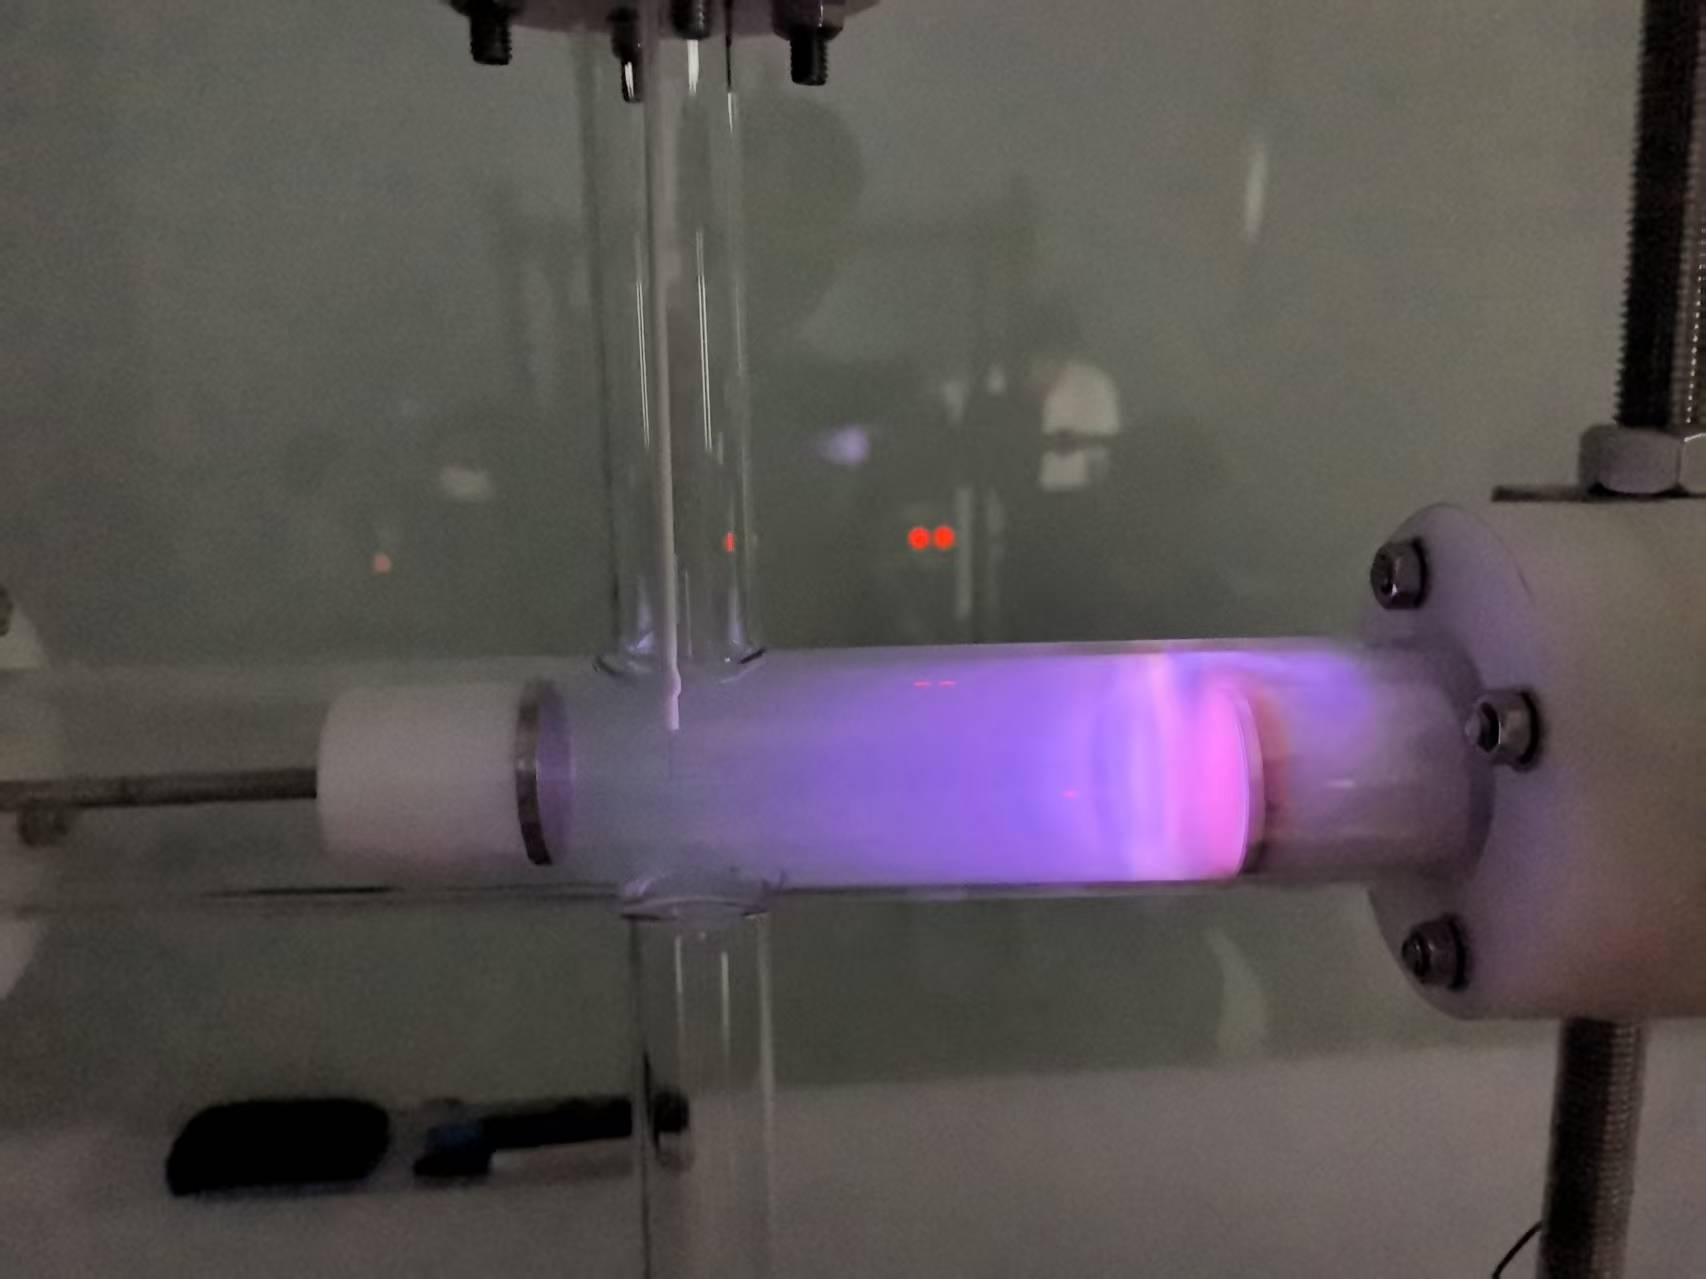
\includegraphics[width=\linewidth,keepaspectratio]{10Pa_异常辉光放电.jpg}
    \caption{异常辉光放电}
  \end{subfigure}
  \caption{10\,Pa下气体放电各阶段形貌}
  \label{fig:disch10}
\end{figure*}

\begin{figure*}[htbp]
  \centering
  \begin{subfigure}{0.32\textwidth}
    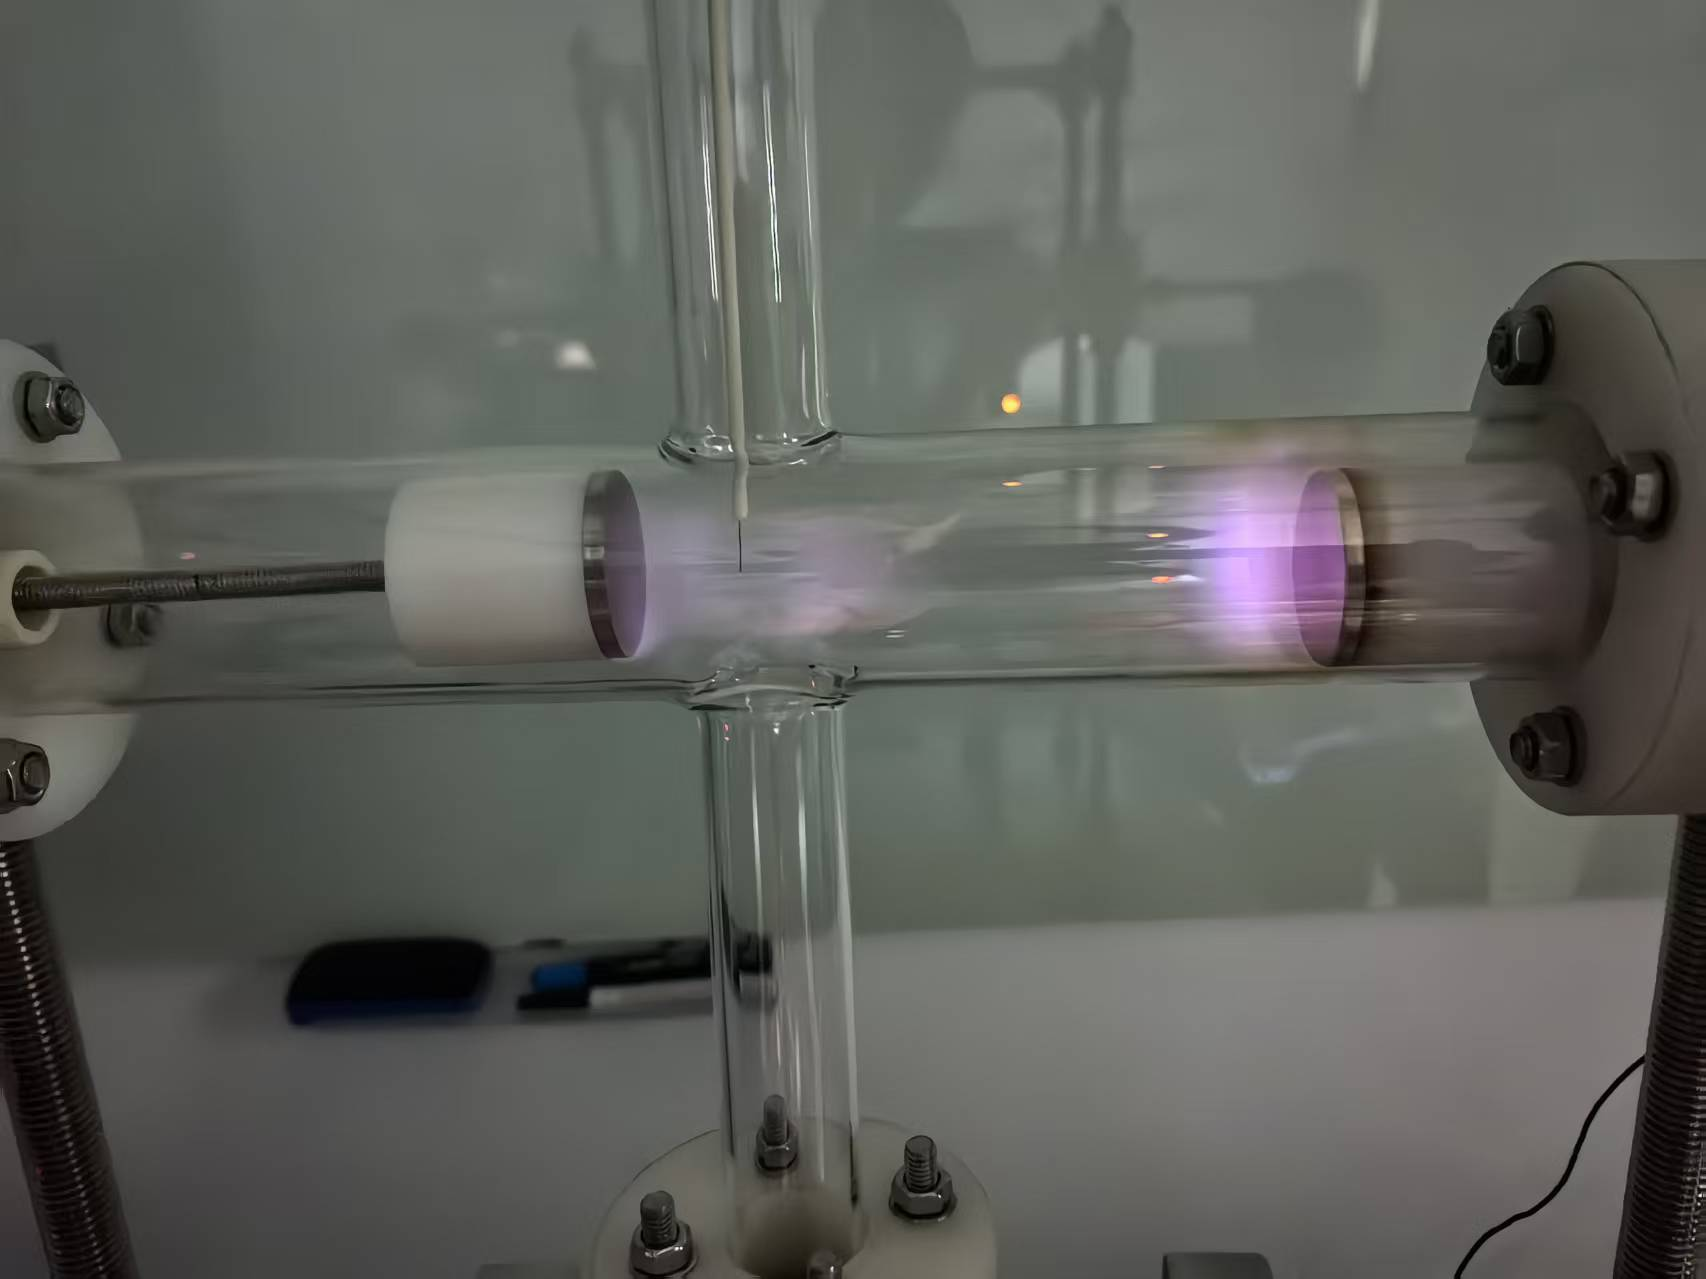
\includegraphics[width=\linewidth,keepaspectratio]{15Pa_汤生放电.jpg}
    \caption{汤生放电}
  \end{subfigure}\hfill
  \begin{subfigure}{0.32\textwidth}
    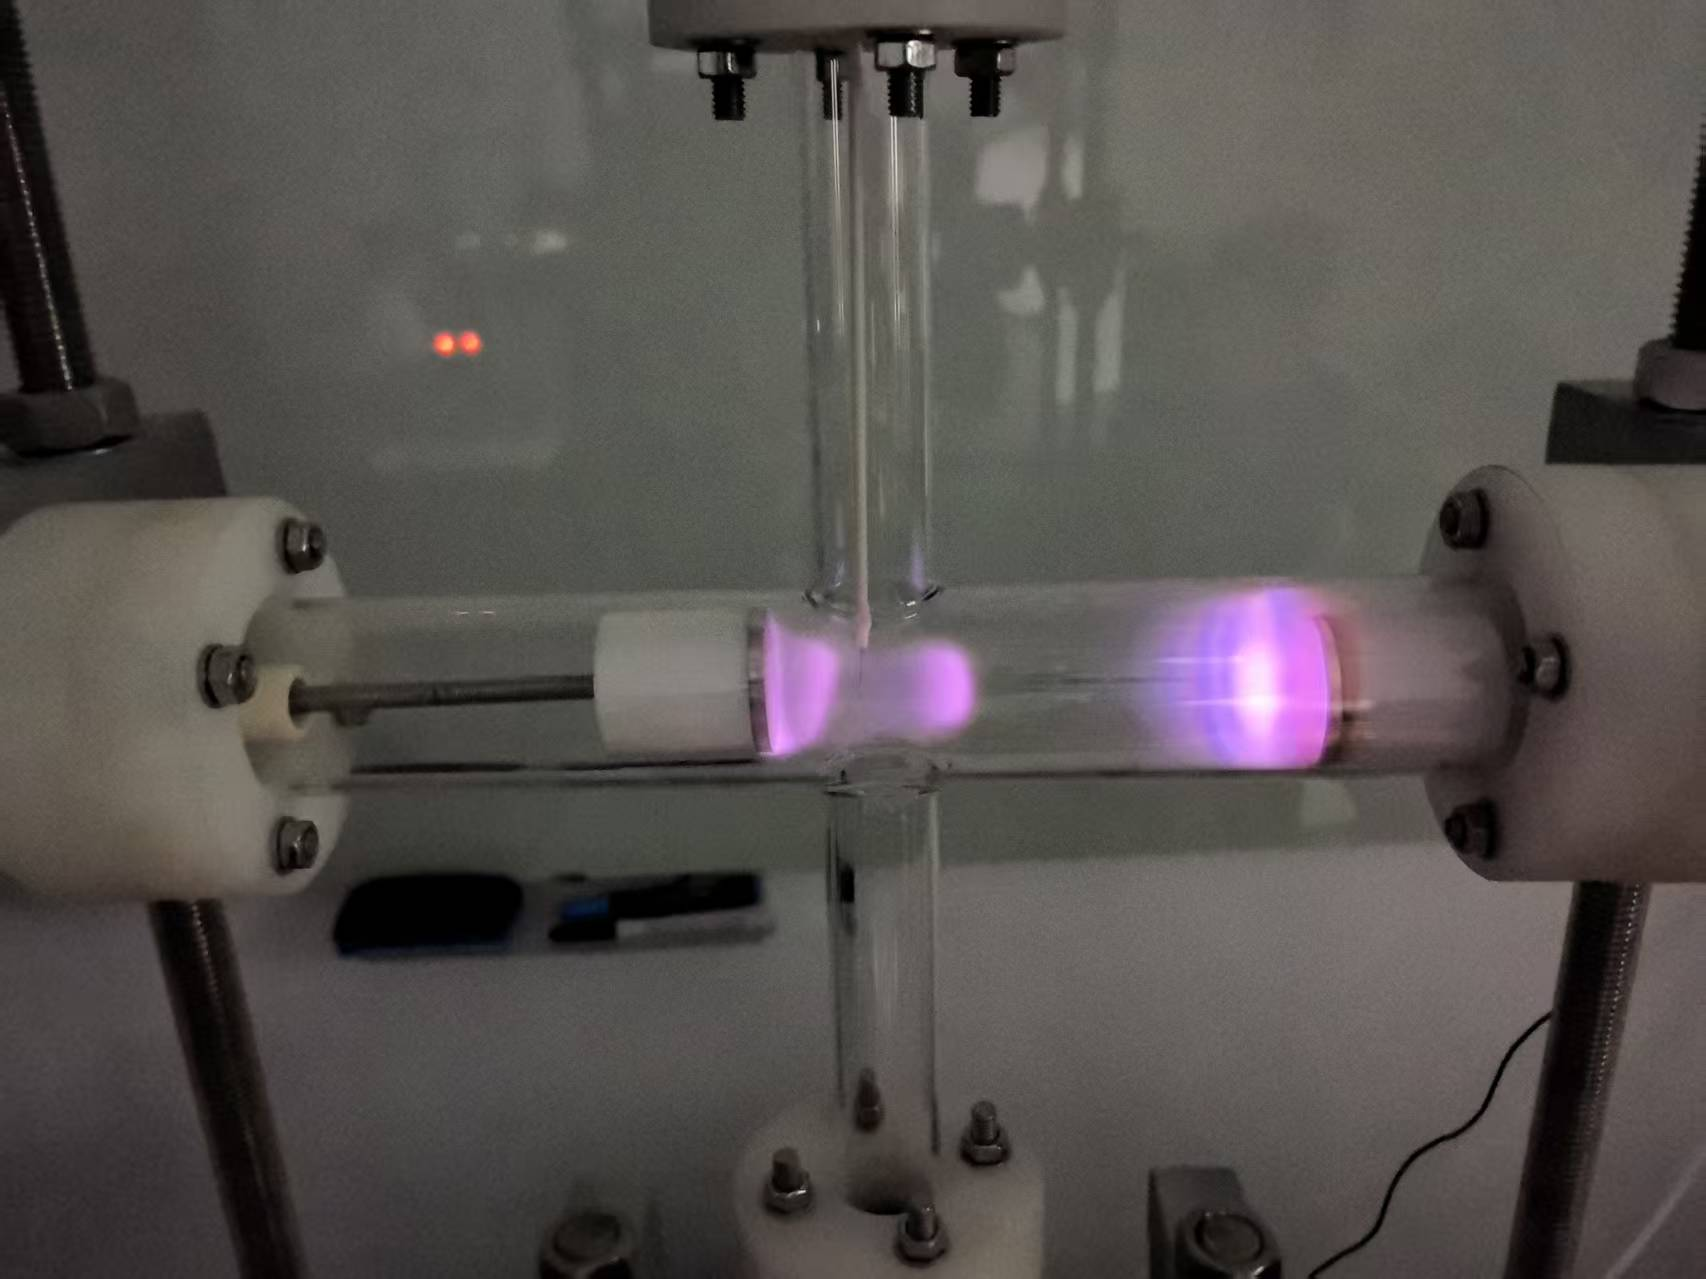
\includegraphics[width=\linewidth,keepaspectratio]{15Pa_正常辉光放电.jpg}
    \caption{正常辉光放电}
  \end{subfigure}\hfill
  \begin{subfigure}{0.32\textwidth}
    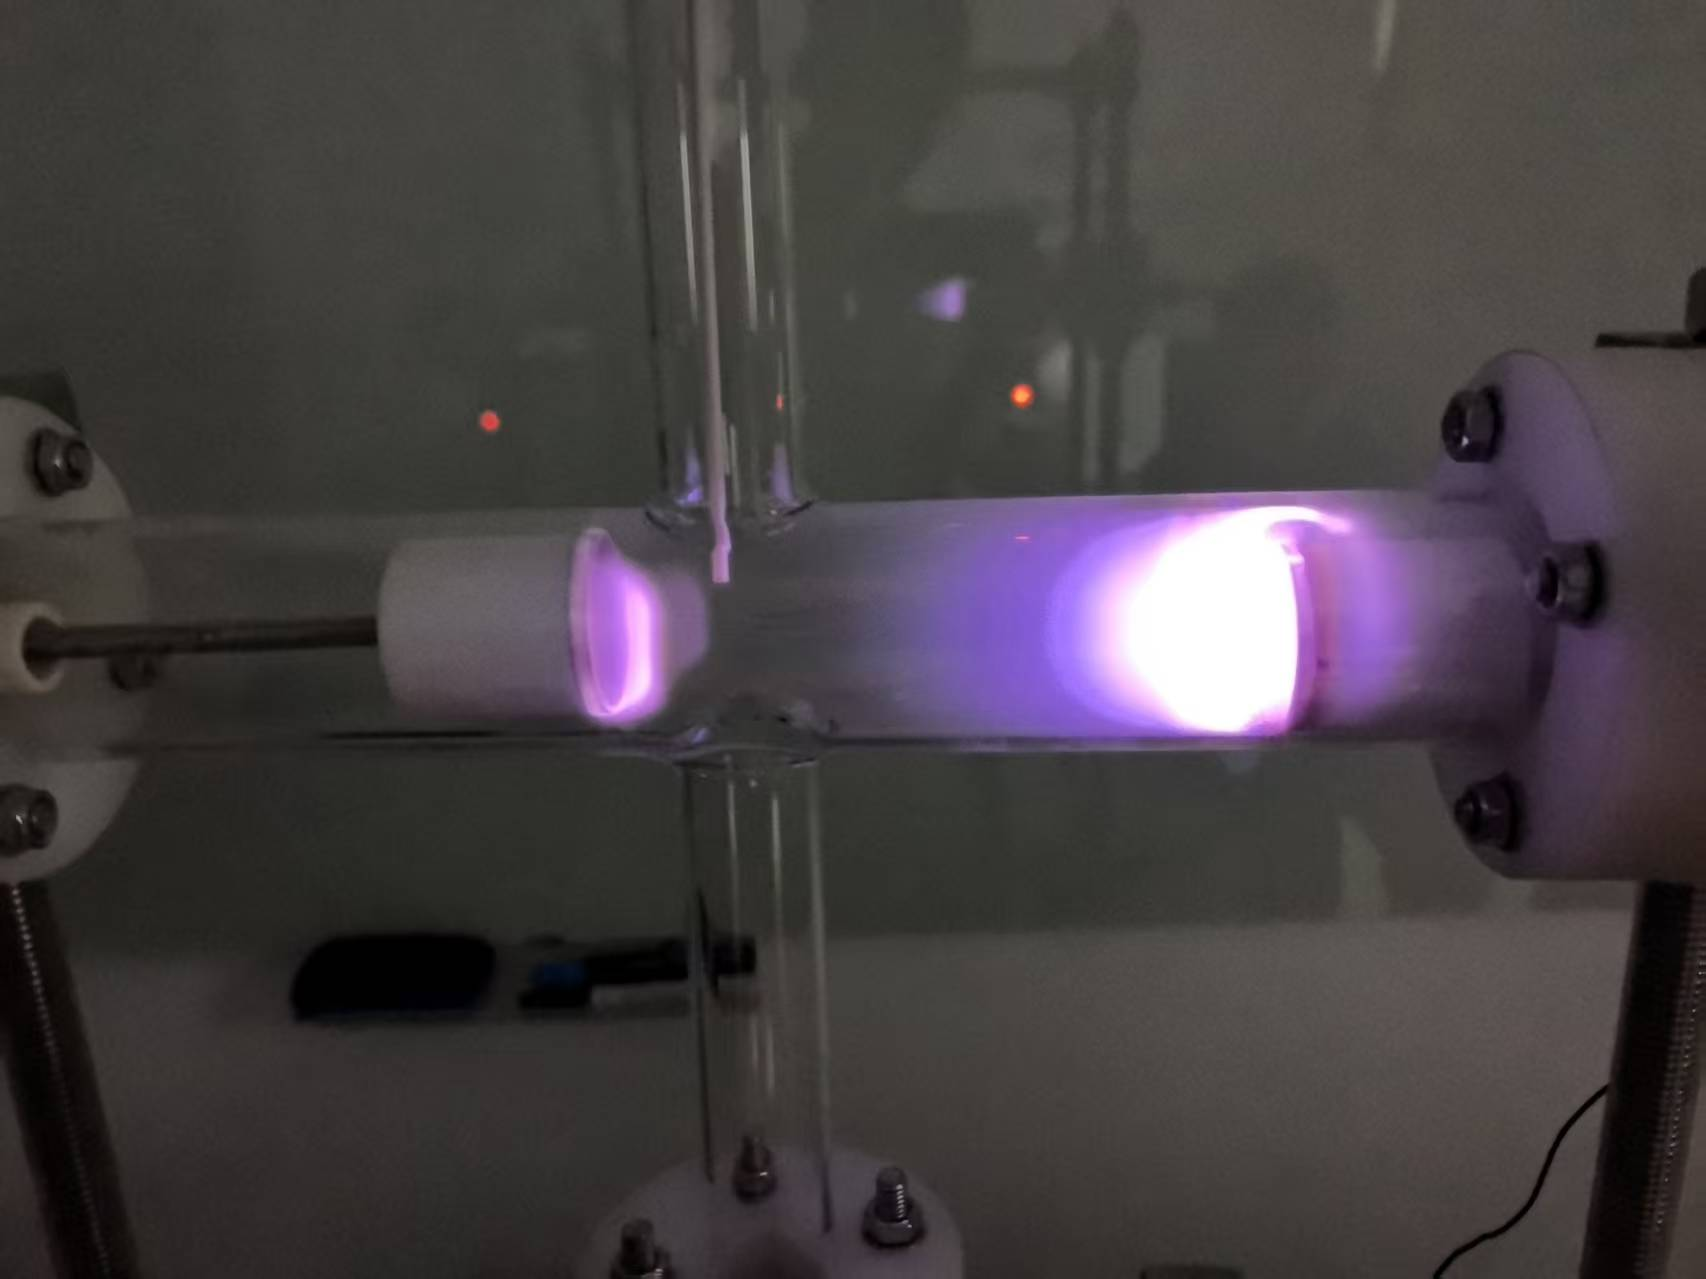
\includegraphics[width=\linewidth,keepaspectratio]{15Pa_异常辉光放电.jpg}
    \caption{异常辉光放电}
  \end{subfigure}
  \caption{15\,Pa下气体放电各阶段形貌}
  \label{fig:disch15}
\end{figure*}

\begin{figure*}[htbp]
  \centering
  \begin{subfigure}{0.32\textwidth}
    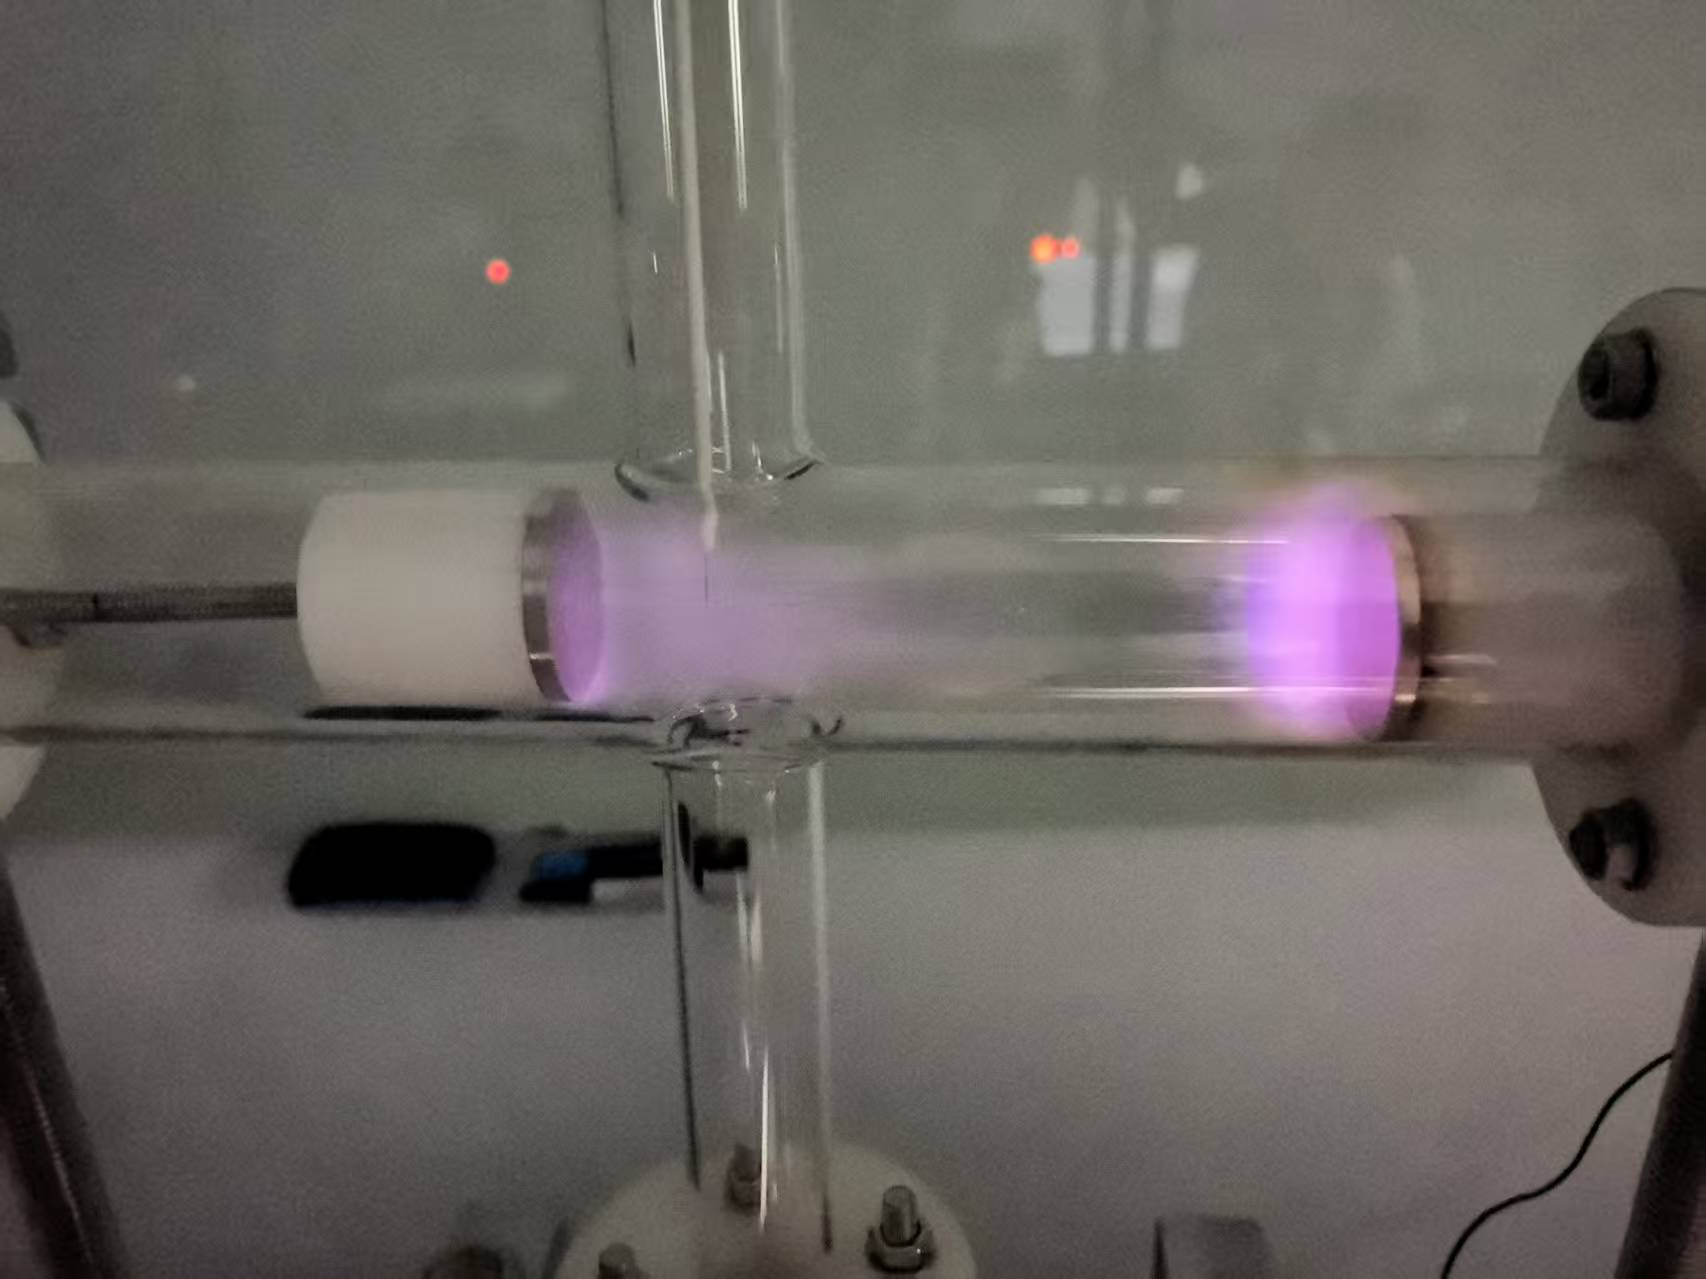
\includegraphics[width=\linewidth,keepaspectratio]{20Pa_汤生放电.jpg}
    \caption{汤生放电}
  \end{subfigure}\hfill
  \begin{subfigure}{0.32\textwidth}
    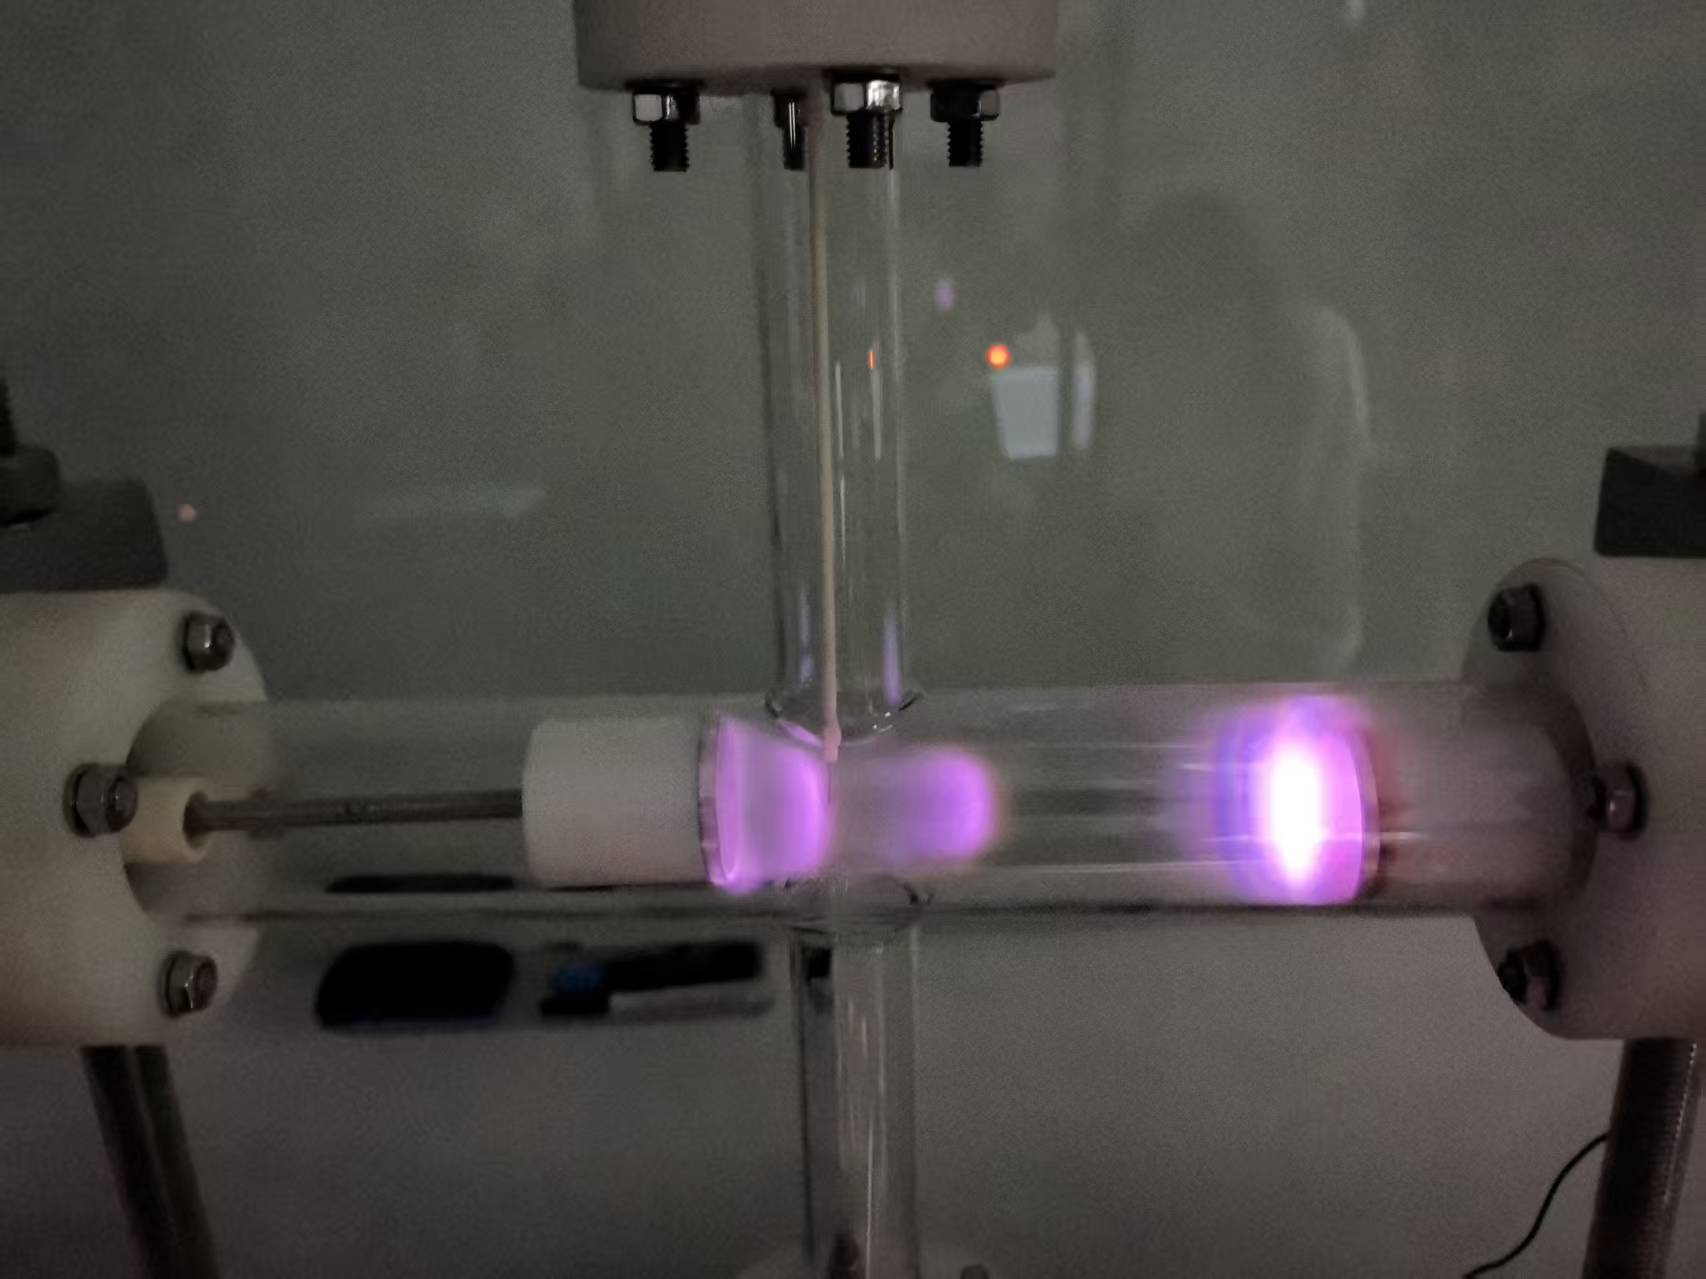
\includegraphics[width=\linewidth,keepaspectratio]{20Pa_正常辉光放电.jpg}
    \caption{正常辉光放电}
  \end{subfigure}\hfill
  \begin{subfigure}{0.32\textwidth}
    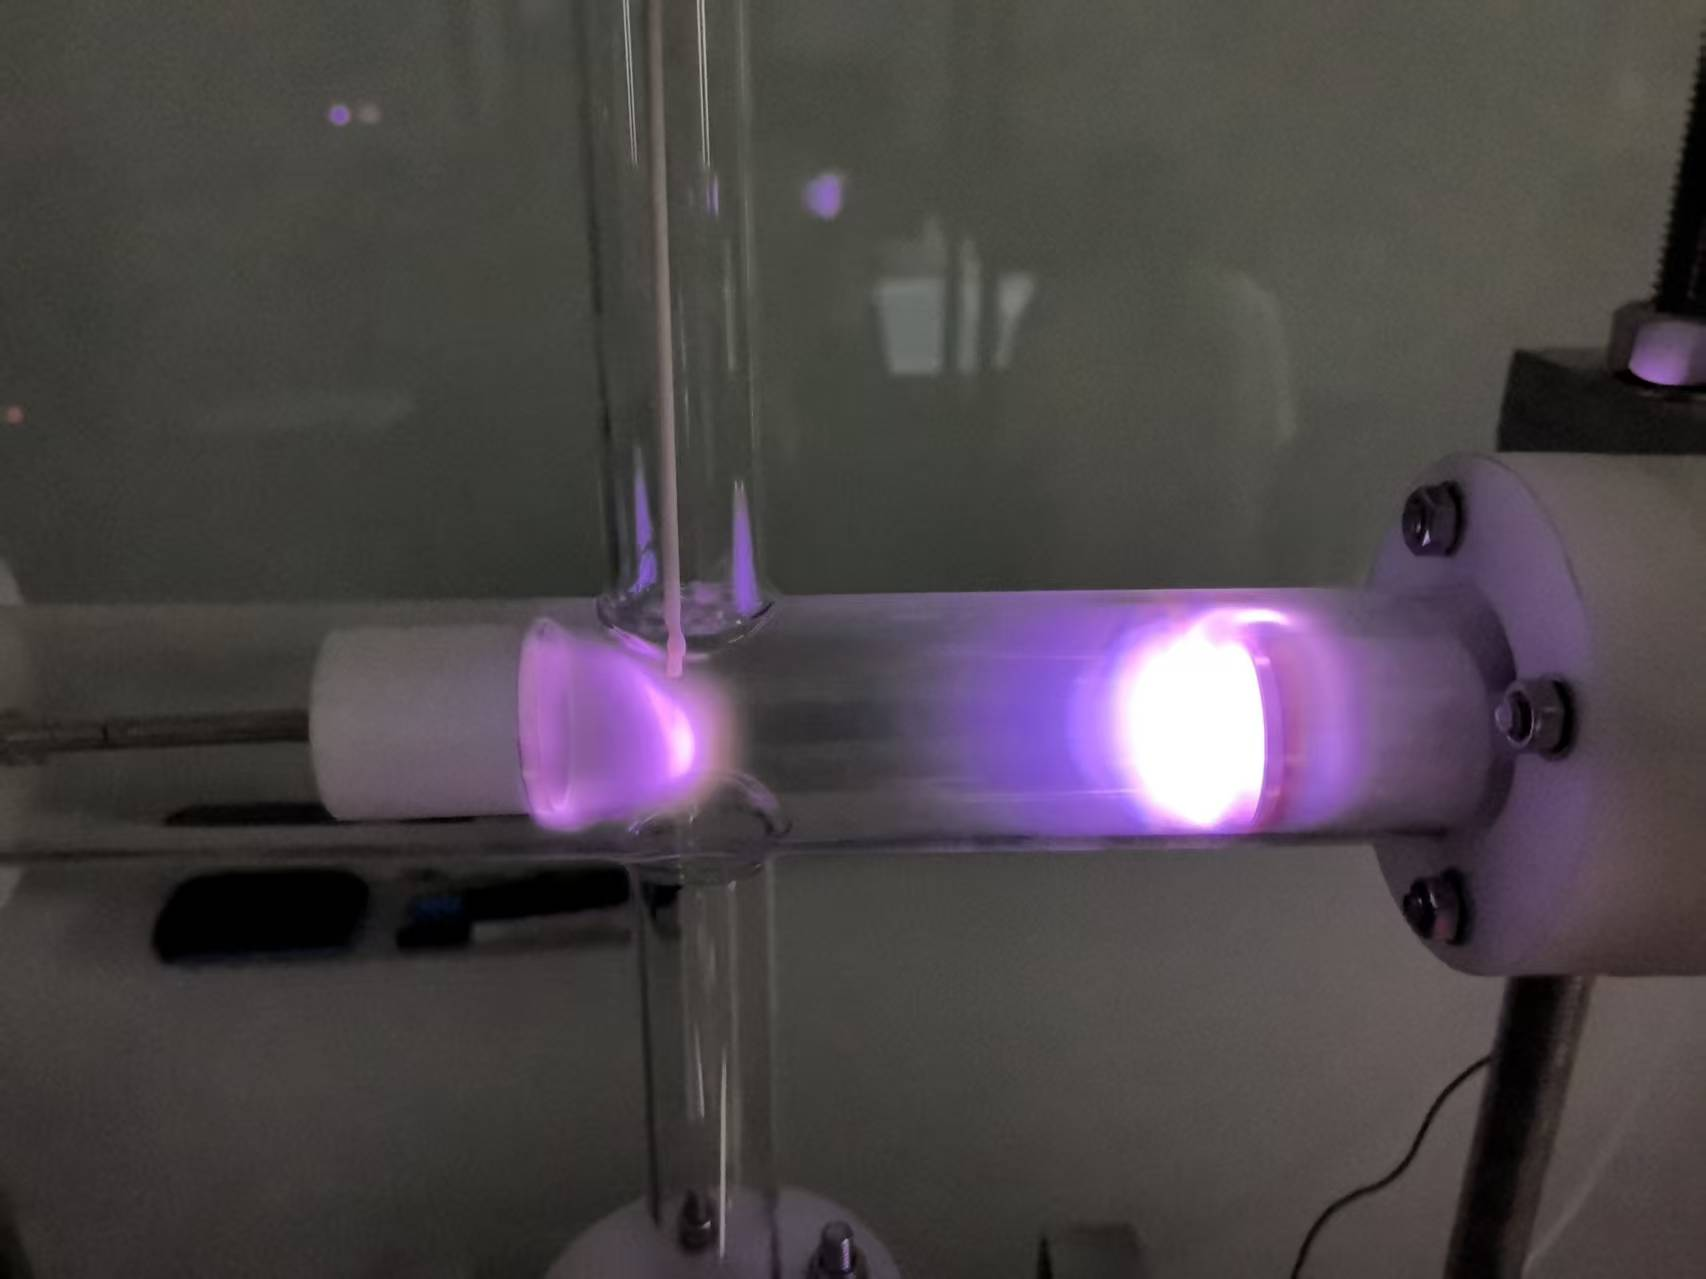
\includegraphics[width=\linewidth,keepaspectratio]{20Pa_异常辉光放电.jpg}
    \caption{异常辉光放电}
  \end{subfigure}
  \caption{20\,Pa下气体放电各阶段形貌}
  \label{fig:disch20}
\end{figure*}

\begin{figure*}[htbp]
  \centering
  \begin{subfigure}{0.32\textwidth}
    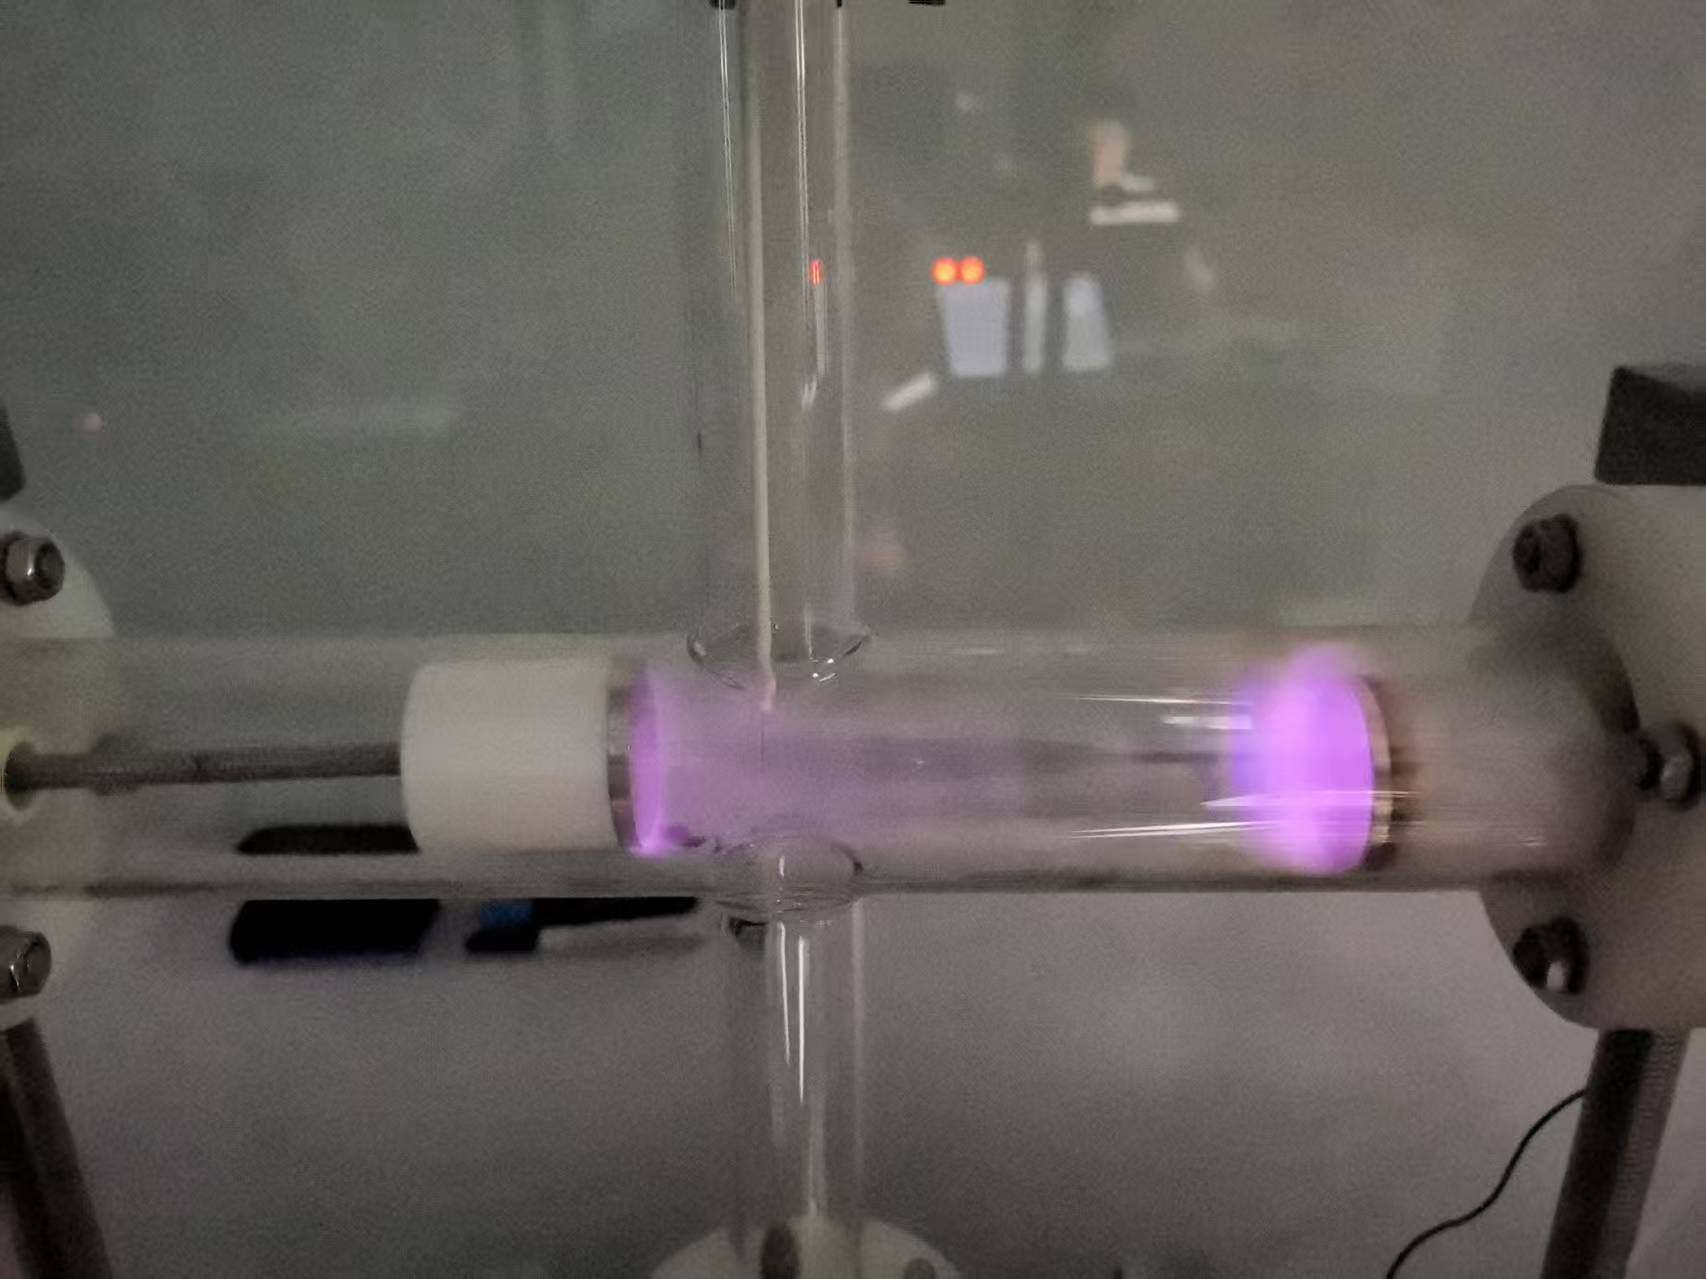
\includegraphics[width=\linewidth,keepaspectratio]{25Pa_汤生放电.jpg}
    \caption{汤生放电}
  \end{subfigure}\hfill
  \begin{subfigure}{0.32\textwidth}
    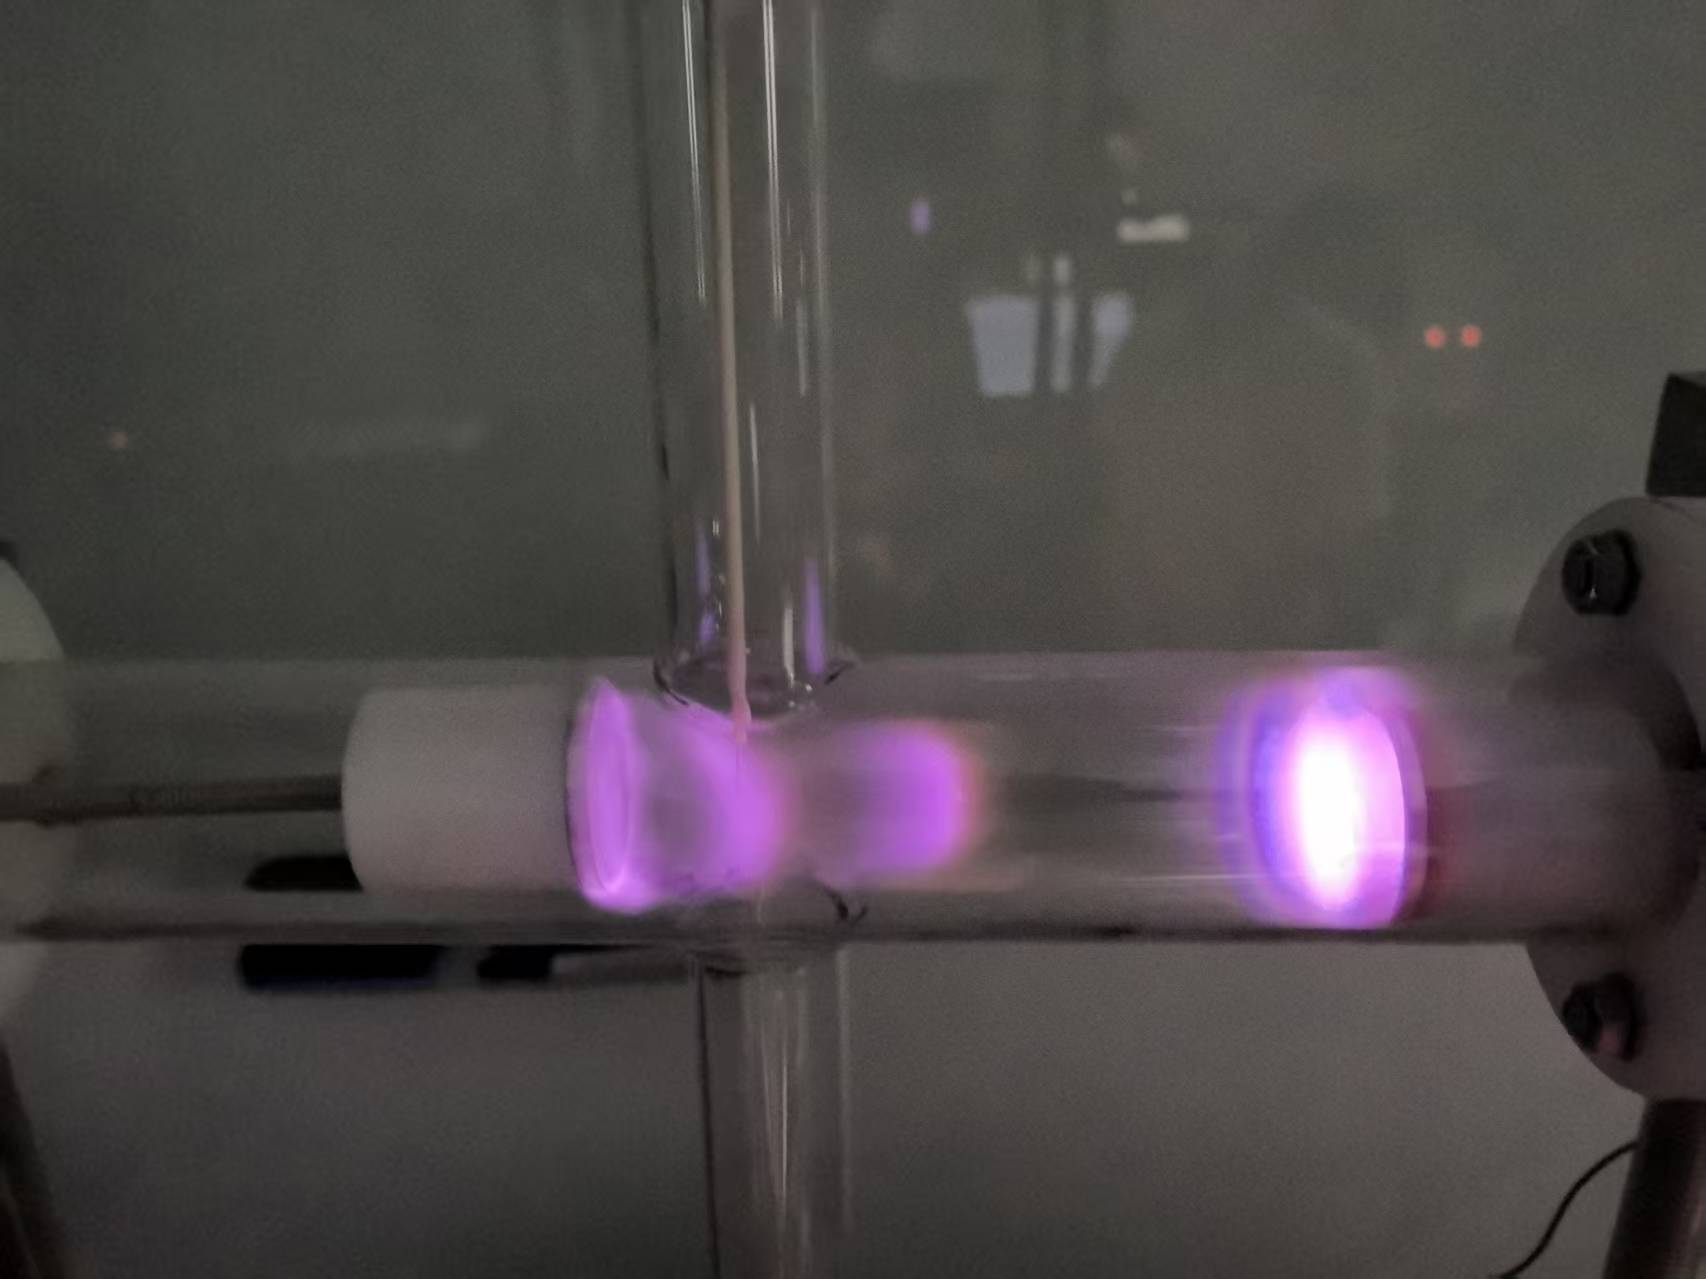
\includegraphics[width=\linewidth,keepaspectratio]{25Pa_正常辉光放电.jpg}
    \caption{正常辉光放电}
  \end{subfigure}\hfill
  \begin{subfigure}{0.32\textwidth}
    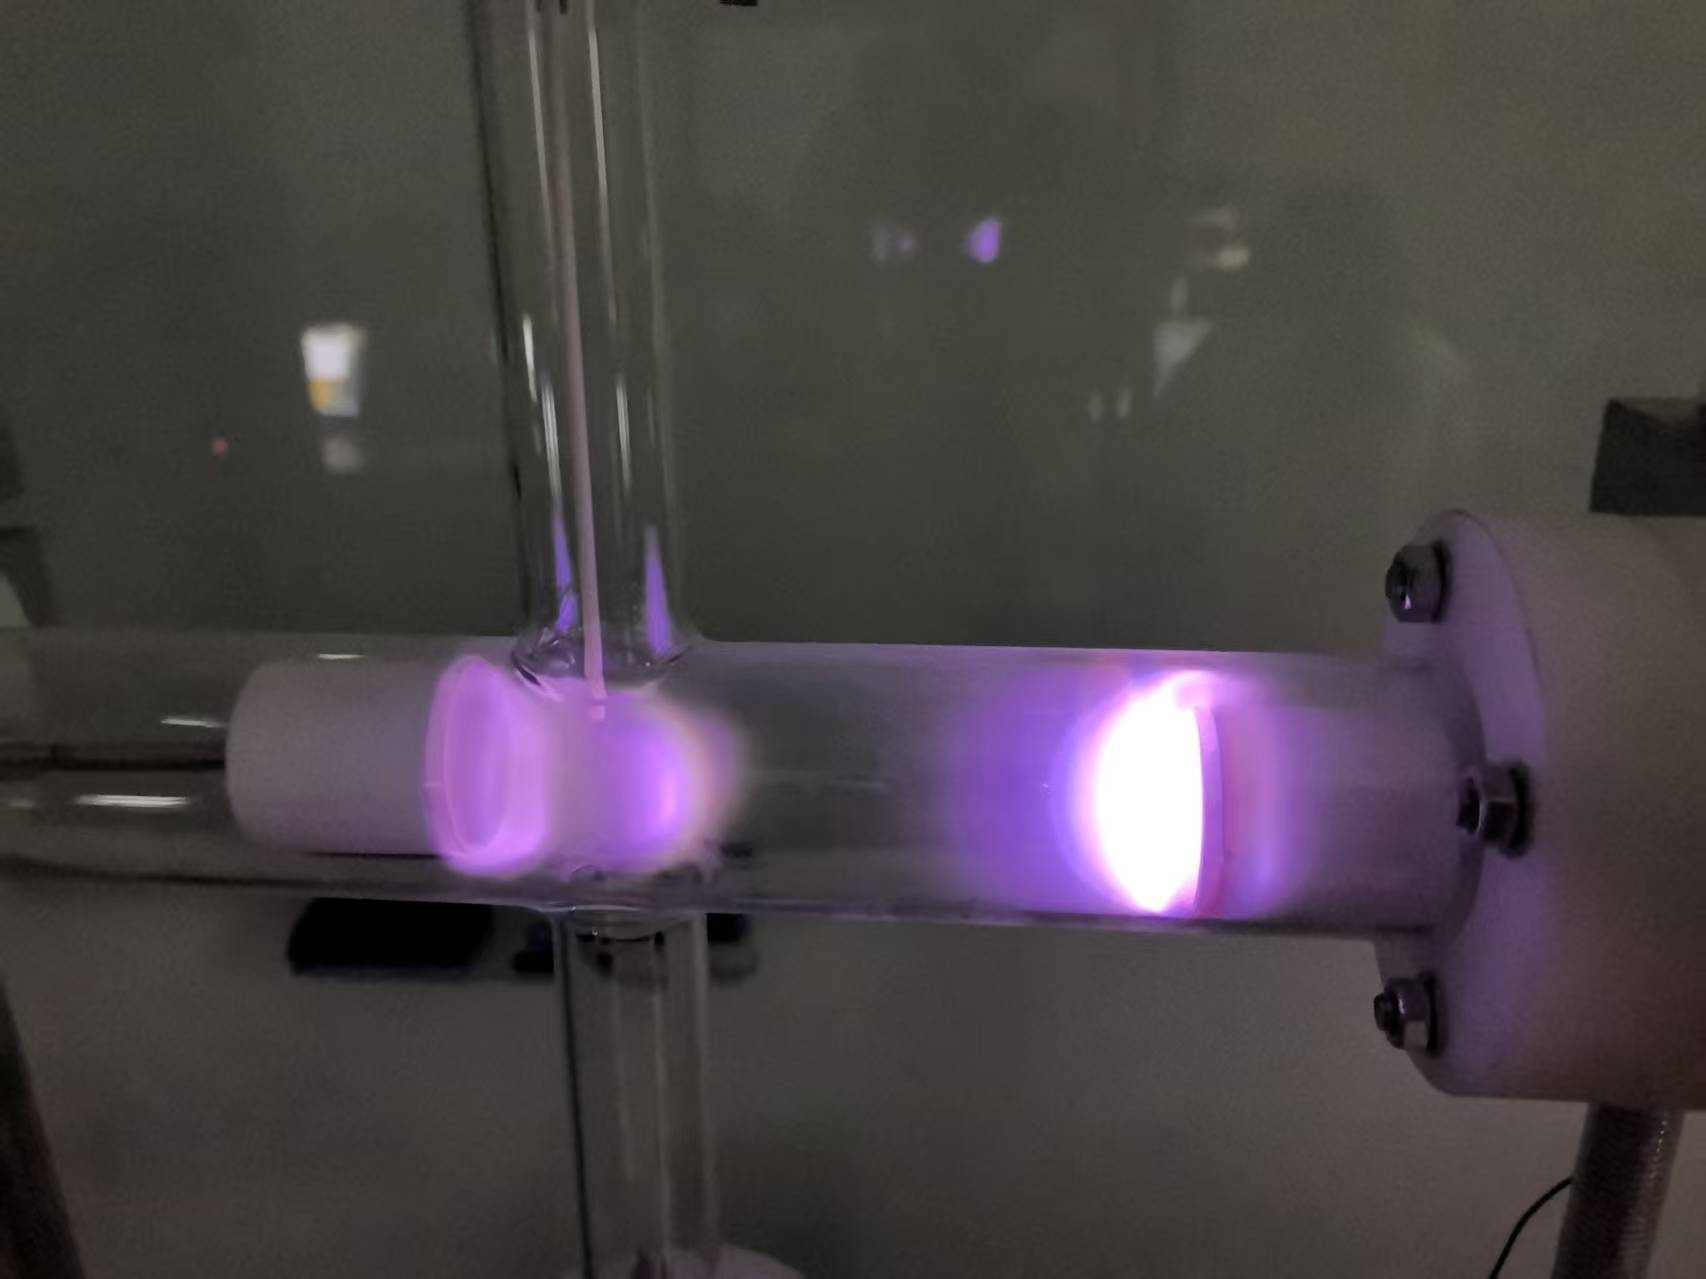
\includegraphics[width=\linewidth,keepaspectratio]{25Pa_异常辉光放电.jpg}
    \caption{异常辉光放电}
  \end{subfigure}
  \caption{25\,Pa下气体放电各阶段形貌}
  \label{fig:disch25}
\end{figure*}

\subsection{等离子体诊断结果}

图\,\ref{fig:iv_probe}\,给出了15、17、19\,Pa下朗缪尔探针的I-V全曲线。
三条曲线均呈现典型的三段式结构：大负压段（$U_p\ll V_f$）为离子饱和区，电流约为$-4$\,\si{\micro\ampere}；
中间过渡区电子电流随$U_p$指数增长；高压段（$U_p>V_p$）电子电流趋于饱和。

\begin{figure*}[htbp]
  \centering
  \begin{tikzpicture}
  \begin{axis}[
    ivplot,
    title={不同气压下朗缪尔探针I-V特性曲线},
    legend entries={15\,Pa, 17\,Pa, 19\,Pa},
    xmin=-105, xmax=105,
    ymin=-15, ymax=640,
  ]
    % ---- 15 Pa ----
    \addplot[mark=none,blue,thick] coordinates {
      (-98.4,-4)(-93.3,-3)(-88,-3)(-83,-3)(-78,-3)(-73,-2)(-67.9,-2)
      (-63,-2)(-58,-1)(-53,-1)(-48,-1)(-43,-1)(-38,0)(-33,0)(-28,0)
      (-23,0)(-18,1)(-13,2)(-8,5)(-6,7)(-4,9)(-3,11)(-2,12)(-1,14)
      (0,15)(0.8,17)(1.6,18)(2.5,20)(3.2,22)(4.2,24)(5.2,26)(6.1,28)
      (6.9,30)(7.7,32)(8.7,34)(9.5,36)(10,38)(10.9,40)(11.5,42)(12,44)
      (12.7,46)(13.3,48)(13.7,50)(14.1,52)(14.7,55)(15.4,58)(16.1,61)
      (16.5,64)(17,67)(17.5,70)(18,73)(18.3,76)(18.7,79)(19.1,82)
      (19.4,85)(19.8,88)(20.2,92)(20.7,95)(21.1,98)(21.6,101)(22,104)
      (22.5,107)(22.8,115)(23.2,119)(23.5,122)(23.8,126)(24.1,129)
      (24.4,133)(24.9,141)(25.2,145)(25.6,150)(25.8,155)(26.1,161)
      (26.5,167)(26.8,175)(27.3,181)(27.7,187)(28,193)(28.4,198)
      (28.8,198)(29.2,203)(29.5,208)(30.1,214)(30.7,221)(31.3,228)
      (32.2,233)(32.8,241)(33.3,248)(34,253)(34.9,260)(35.8,272)
      (36.3,276)(36.9,285)(37.2,290)(37.7,300)(37.8,308)(38.2,322)
      (38.5,333)(39,344)(39.5,356)(40.1,369)(40.8,381)(41.5,394)
      (42.2,405)(42.8,414)(43.8,424)(45.1,432)(46.2,440)(48.5,451)
      (52.4,461)(56.9,471)(61.4,473)(66,478)(70.9,496)(74.9,501)
      (80.2,503)(85.0,510)(90.1,516)(94.6,520)(100,525)
    };
    % ---- 17 Pa ----
    \addplot[mark=none,red,thick] coordinates {
      (-97.6,-4)(-91.9,-3)(-87.2,-3)(-82.0,-3)(-78,-3)(-72,-2)(-68,-2)
      (-62,-2)(-58,-2)(-52,-1)(-48,-1)(-42,-1)(-28,0)(-32,0)(-28,0)
      (-22,1)(-17,3)(-12,5)(-7,9)(-1.2,14)(2.3,19)(4.8,24)(6.7,29)
      (8.3,34)(9.6,39)(10.6,44)(11.8,49)(12.6,53)(13.5,59)(14.3,64)
      (14.9,69)(15.6,74)(16.3,81)(17.1,86)(17.6,91)(18.4,97)(19,101)
      (19.7,107)(20.3,114)(20.8,120)(21.3,128)(21.9,127)(22.6,146)
      (23.6,155)(23.9,163)(24.6,172)(25,183)(25.3,194)(26.5,207)
      (28,217)(29.4,226)(31.1,233)(32.8,240)(33.5,246)(34.3,253)
      (35.4,264)(36.4,277)(37.2,299)(37.9,307)(38.4,322)(39.1,344)
      (39.5,361)(40,380)(40.3,399)(40.7,415)(41.5,440)(42.5,457)
      (43.2,469)(45.1,477)(47.6,493)(51.7,505)(56.3,510)(59.9,513)
      (65.1,516)(69.8,522)(74.9,531)(80.2,534)(85,536)(90,541)
      (95.1,548)(100.3,551)
    };
    % ---- 19 Pa ----
    \addplot[mark=none,green!55!black,thick] coordinates {
      (-97.3,-4)(-92.2,-4)(-86.9,-3)(-81.9,-3)(-77,-3)(-71.9,-3)
      (-66.9,-2)(-61.8,-2)(-58,-2)(-51.9,-1)(-47.1,-1)(-42,-1)
      (-37,0)(-32.1,0)(-27,1)(-21.9,2)(-17,4)(-11.9,6)(-7,9)
      (-2,14)(1,19)(2.8,23)(4.8,28)(6.4,34)(7.7,39)(9.2,45)(10,50)
      (11.1,56)(12,61)(12.8,66)(13.8,74)(14.5,80)(15.7,89)(16.9,97)
      (17.9,107)(18.8,116)(19.6,127)(20.3,138)(20.9,149)(21.6,163)
      (22.2,175)(22.8,185)(23.3,194)(24,210)(24.6,233)(25.7,245)
      (27.1,252)(28,254)(29,259)(30.3,263)(31.8,270)(33.3,281)
      (34.1,288)(35.3,302)(36.4,316)(37.2,333)(37.9,353)(38.5,370)
      (39.1,395)(39.5,412)(40,433)(40.4,453)(40.9,473)(41.5,492)
      (42.1,506)(42.9,524)(44.3,541)(46.1,551)(48.2,562)(50.7,572)
      (53.6,578)(56.5,583)(60.6,584)(64.1,589)(66.3,590)(71.4,593)
      (76.1,600)(81.4,605)(86.2,612)(91,619)(96.3,627)(100.9,629)
    };
  \end{axis}
  \end{tikzpicture}
  \caption{不同气压下朗缪尔探针I-V特性曲线。负压区为离子饱和区，
           中间过渡区电流指数增长，高压区为电子饱和区。}
  \label{fig:iv_probe}
\end{figure*}

图\,\ref{fig:lniv}\,给出了过渡区的$\ln I_p$—$U_p$图及线性拟合直线。
各气压下过渡区均呈现良好的线性关系，验证了麦克斯韦速度分布假设。

\begin{figure}[H]
  \centering
  \begin{tikzpicture}
  \begin{axis}[
    lnivplot,
    title={过渡区 $\ln I_p$—$U_p$ 线性拟合},
    legend entries={15\,Pa数据, 15\,Pa拟合, 17\,Pa数据, 17\,Pa拟合, 19\,Pa数据, 19\,Pa拟合},
    xmin=-10, xmax=25,
    ymin=0, ymax=6,
  ]
    % ---- 15 Pa data (transition region) ----
    \addplot[only marks, mark=*, mark size=0.8pt, blue] coordinates {
      (-8,1.61)(-6,1.95)(-4,2.20)(-3,2.40)(-2,2.48)(-1,2.64)(0,2.71)
      (0.8,2.83)(1.6,2.89)(2.5,3.00)(3.2,3.09)(4.2,3.18)(5.2,3.26)
      (6.1,3.33)(6.9,3.40)(7.7,3.47)(8.7,3.53)(9.5,3.58)(10,3.64)
      (10.9,3.69)(11.5,3.74)(12,3.78)(12.7,3.83)(13.3,3.87)(13.7,3.91)
      (14.1,3.95)(14.7,4.01)(15.4,4.06)(16.1,4.11)(16.5,4.16)(17,4.21)
      (17.5,4.25)(18,4.29)(18.3,4.33)(18.7,4.37)(19.1,4.41)(19.4,4.44)
      (19.8,4.48)(20.2,4.52)(20.7,4.55)
    };
    % 15 Pa fit: y = 0.1027x + 2.431
    \addplot[blue, thick, domain=-8:20.7] {0.1027*x + 2.431};

    % ---- 17 Pa data ----
    \addplot[only marks, mark=square*, mark size=0.8pt, red] coordinates {
      (-7,2.20)(-1.2,2.64)(2.3,2.94)(4.8,3.18)(6.7,3.37)(8.3,3.53)
      (9.6,3.66)(10.6,3.78)(11.8,3.89)(12.6,3.97)(13.5,4.08)(14.3,4.16)
      (14.9,4.23)(15.6,4.30)(16.3,4.39)(17.1,4.45)(17.6,4.51)(18.4,4.57)
      (19,4.62)(19.7,4.67)(20.3,4.74)(20.8,4.79)(21.3,4.85)
    };
    % 17 Pa fit: y = 0.0930x + 2.848
    \addplot[red, thick, domain=-7:21.3] {0.0930*x + 2.848};

    % ---- 19 Pa data ----
    \addplot[only marks, mark=triangle*, mark size=0.8pt, green!55!black] coordinates {
      (-7,2.20)(-2,2.64)(1,2.94)(2.8,3.14)(4.8,3.33)(6.4,3.53)
      (7.7,3.66)(9.2,3.81)(10,3.91)(11.1,4.03)(12,4.11)(12.8,4.19)
      (13.8,4.30)(14.5,4.38)(15.7,4.49)(16.9,4.57)(17.9,4.67)
      (18.8,4.75)(19.6,4.84)
    };
    % 19 Pa fit: y = 0.0995x + 2.894
    \addplot[green!55!black, thick, domain=-7:19.6] {0.0995*x + 2.894};
  \end{axis}
  \end{tikzpicture}
  \caption{过渡区$\ln I_p$—$U_p$线性拟合。实线为各气压对应的线性拟合直线，
           斜率用于计算电子温度$T_e$。}
  \label{fig:lniv}
\end{figure}

由线性拟合斜率及式(1)(2)计算所得等离子体参数汇总于表\,\ref{tab:plasma}。
探针有效面积取$A=\pi DL=\pi\times0.12\times10^{-3}\times10\times10^{-3}
=3.77\times10^{-6}$\,m$^2$。

\begin{table}[H]
\centering
\caption{各气压下等离子体诊断参数}
\label{tab:plasma}
\begin{tabular}{lp{1.5cm}p{1.5cm}p{1.5cm}}
\toprule
参数 & 15\,Pa & 17\,Pa & 19\,Pa \\
\midrule
$V_f$\,(\si{\volt})                             & $-28$      & $-28$      & $-32$      \\
$V_p$\,(\si{\volt})                             & $\approx48$ & $\approx47$ & $\approx46$ \\
斜率$k$\,(\si{\per\volt})                       & $0.103$    & $0.093$    & $0.100$    \\
$kT_e$\,(\si{\electronvolt})                    & $9.7$      & $10.8$     & $10.1$     \\
$I_\text{sat}$\,(\si{\micro\ampere})            & $470$      & $510$      & $580$      \\
$n_e$\,($10^{15}$\,m$^{-3}$)                   & $1.49$     & $1.54$     & $1.81$     \\
$\lambda_D$\,(\si{\milli\meter})                & $0.60$     & $0.63$     & $0.60$     \\
\bottomrule
\end{tabular}
\end{table}

由表可见，随气压升高，等离子体密度增大，这与气压升高后气体分子数密度增大、
碰撞电离频率提高相符。三个气压下电子温度$kT_e$均在10\,eV量级，变化不大，
说明在本实验气压范围内正柱区的电子能量分布较为稳定。
德拜长度均在0.6\,mm左右，远大于探针针尖直径$D=0.12$\,mm，
满足朗缪尔探针测量要求（探针尺寸$<\lambda_D$），测量结果可信。

%%%%%%%%%%%%%%%%%%%%%%%%%%%%%%%%%%%%%%%%%%%%%%%%%%%%%%%%%%%%
\section{思考与分析}

\begin{enumerate}
  \item \textbf{正常辉光放电阶段，随电流增大，电压为何基本不变？}\\[0.3em]
  正常辉光放电时，阴极面只有部分区域参与放电，放电所需的维持电压由气体类型和压强决定，
  与放电面积无关。当外电路电流增大时，放电斑点面积等比例扩大，
  单位面积的电流密度（即离子轰击强度与二次电子发射率）保持不变，
  因此放电管两端的维持电压保持近似恒定。直至阴极面全部被放电斑点覆盖，
  电流不能再通过扩面方式增大，才进入异常辉光放电阶段。

  \item \textbf{朗缪尔探针的悬浮电位为何通常为负值？}\\[0.3em]
  在等离子体中，电子质量远小于离子，热运动速度远大于离子（约为$v_e/v_i\sim\sqrt{m_i/m_e}\gtrsim100$倍）。
  当探针处于悬浮状态（不接入外电路）时，初始瞬间到达探针的电子流远大于离子流，
  探针迅速积累负电荷，形成一个负的接触电位，使探针周围形成排斥电子的势垒。
  当排斥势使到达探针的电子流与离子流恰好相等（净电流为零）时，
  探针达到稳定的悬浮电位，此时$V_f<0$（以阳极/地为参考）。

  \item \textbf{气体压强对放电V-I特性曲线有何影响？}\\[0.3em]
  由图\,\ref{fig:vi_all}可见，随气压升高：（1）正常辉光放电的维持电压降低，
  最小放电维持电压（对应V-I曲线最低点）也随之降低，这符合帕邢定律——
  压强增大时电子平均自由程减小，所需电场强度降低；
  （2）正常辉光放电对应的电流范围向更小的电流移动，
  高电流段（异常辉光放电）的V-I斜率增大（阻抗增大），
  这与高压下带电粒子碰撞损失增加有关。

  \item \textbf{如何从I-V曲线确定等离子体空间电位$V_p$？}\\[0.3em]
  等离子体空间电位$V_p$是探针周围鞘层消失的临界点。实验上，
  $V_p$对应I-V曲线从指数增长（过渡区）转变为饱和（或线性增长）的拐点，
  即$\text{d}^2I/\text{d}U_p^2=0$处。实际操作中可取$\ln I_p$—$U_p$
  图中线性区终止处对应的电位，或者取I-V曲线中斜率（$\text{d}I/\text{d}U_p$）
  达到最大值处的电位作为$V_p$的估计值。

  \item \textbf{解释气体放电中的空间电荷、等离子体及弹性碰撞、非弹性碰撞的概念。}\\[0.3em]

  \textbf{空间电荷}：放电管内部，由于电子迁移率远大于正离子，
  在阴极暗区附近会形成正离子堆积，而在负辉区附近则有电子积累，
  这种局部净电荷称为空间电荷。空间电荷会显著畸变管内的电场分布——
  阴极位降区的强电场正是由大量正空间电荷维持的，它为电子提供加速所需的能量。

  \textbf{等离子体}：当放电进入正柱区后，电子和正离子的浓度近似相等
  （约$10^{15}$—$10^{16}$\,m$^{-3}$），宏观上呈现电中性，称为等离子体（物质第四态）。
  等离子体具有良好的导电性，内部几乎无宏观电场，粒子以无规热运动（扩散运动）为主。
  描述等离子体最小尺度的特征量为德拜长度$\lambda_D$，
  只有大于$\lambda_D$的尺度才可视为严格意义上的等离子体。

  \textbf{弹性碰撞}：碰撞前后粒子的内部状态不变，仅发生动能和动量的交换。
  由于电子质量远小于气体分子质量，单次弹性碰撞中电子传递给分子的能量极少
  （约$2m_e/M$量级），但多次弹性碰撞累积效应使气体温度缓慢升高。
  低能电子（能量低于激发能阈值）主要以弹性碰撞方式与气体分子相互作用。

  \textbf{非弹性碰撞}：碰撞后粒子内部状态发生改变，电子的动能转化为分子的内能，
  主要包括：（1）\textbf{激发碰撞}——电子能量足以将分子提升至激发态，
  激发态分子退激时发射光子，这正是辉光放电发光的根本原因；
  （2）\textbf{电离碰撞}——电子能量超过分子电离能，使分子失去一个电子，
  产生新的电子–正离子对，这是维持自持放电（雪崩倍增）的关键过程；
  （3）\textbf{复合与附着}——正离子捕获电子复合为中性粒子，
  或电负性气体分子俘获电子形成负离子，这两类过程使载流子密度降低。
\end{enumerate}

%%%%%%%%%%%%%%%%%%%%%%%%%%%%%%%%%%%%%%%%%%%%%%%%%%%%%%%%%%%%
\clearpage
\onecolumn
\section*{参考文献}

\begin{enumerate}[label={[\arabic*]}]
  \item Chen F F. Langmuir Probe Diagnostics[R]. University of California, Los Angeles, 2003.
  \item Hiden Analytical. Langmuir Probe Manual[M]. 2003.
  \item Plasmart Inc. Probe System Manual[M]. 2004.
  \item 杨津基. 气体放电[M]. 北京: 科学出版社.
  \item 胡志强. 气体电子学[M]. 北京: 电子工业出版社.
  \item 沈阳斯玛特真空科技有限公司. 物理实验——气体放电与等离子体诊断理论基础[M]. 2017.
\end{enumerate}

\clearpage

\section{教师签名页}
\begin{figure}[H]
  \centering
  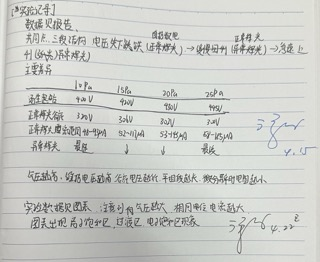
\includegraphics[scale=0.25]{签名.jpeg}
  \caption{教师签名页}
\end{figure}

\end{document}
